\documentclass[oneside, openany] {book}
\usepackage{listings}
\usepackage{minitoc}

\usepackage{hyperref}
\usepackage{parskip}
\usepackage{graphicx}
\usepackage{adjustbox}
\usepackage[utf8]{inputenc}
\usepackage[T1]{fontenc}
\usepackage{xcolor}
\usepackage{caption}
\usepackage{hyperref}
\usepackage{minted}
\usepackage{etoolbox}
\usepackage{imakeidx}
\usepackage{microtype}
\DeclareUnicodeCharacter{2003}{ }
\makeindex[title=Index, intoc]


\graphicspath{ {./images/} }

\tolerance=1
\emergencystretch=\maxdimen
\hyphenpenalty=10000
\hbadness=10000
\AtBeginEnvironment{minted}{%
  \renewcommand{\fcolorbox}[4][]{#4}}
  
 \newminted[CSharp]{csharp}{style=vs}
 
\newcounter{exerciseChapterCounter}
\newcounter{exerciseQuestionCounter}
\setcounter{exerciseChapterCounter}{1}
\setcounter{exerciseQuestionCounter}{0}
   
\newcommand{\exercise}{

    \ifnum \value{chapter}>\value{exerciseChapterCounter} %If the actual chapter value is greater than our previously-defined chapter count variable...
    \stepcounter{exerciseChapterCounter}
    \setcounter{exerciseQuestionCounter}{1}  %Reset exercise counter
\else
    \stepcounter{exerciseQuestionCounter} %Otherwise, if we're still in a chapter, just increase the exercise count
\fi

\section*{Exercise \arabic{exerciseChapterCounter}-\arabic{exerciseQuestionCounter}}

}
\begin{document}

% ---------------------------------------------------------------------------
% Note for GitHub readers:
% Downloading this file is recommended; much of the text is cut off otherwise.
% Otherwise, use the arrow keys to scroll through the document.
% ----------------------------------------------------------------------------

\definecolor{commentcolor}{RGB}{87,166,74}
\definecolor{stringcolor}{RGB}{214,157,133}

\dominitoc
\title{Introduction to Programming for New Developers with C\#}
\date{}
\author{Alexander Summers}
\maketitle
\tableofcontents
\frontmatter
\chapter{Preface}

Welcome to my introductory programming textbook. If you picked this up, you may have a general interest in computer programming but with only knowledge of how to use a computer. If so, you're in the right place -- my primary goal with this book is to take you from ground zero to a solid understanding of programming.

Our primary tool in our journey will be C\#, a programming language created by Microsoft and inspired by several languages, mainly Java and C++. I chose this language for a few reasons:

\begin{itemize}
    \item Extensive documentation -- it's easy to research any aspect of the language due to Microsoft maintaining an extensive set of articles about it.
    \item It's continuously updated by Microsoft to add new features to comply with the increasing needs of programmers.
    \item It is relatively easy to understand in comparison to some other programming languages -- more on that in Chapter 1.
\end{itemize}
For this book, I recommend using a Windows PC. While early chapters of this book will work with MacOS and GNU/Linux computers, we'll soon get into Windows-specific graphical programming. This book will also not provide assistance for setting your development environment in the latter two operating systems.

Ultimately, this book is meant to provide you with a general foundation of computer programming, not just C\#. Chapter 1 in particular emphasizes this point -- it covers the general concepts of modern programming languages. In that sense, much of the early chapters can be thought of as application of those overarching principles through the lens of C\#.

One aspect of this text that is unique is an emphasis o n examples and exercises, which are placed liberally throughout the chapters. These serve not only to reinforce the text but to actively complement it and extend your learning. I recommend completing as many as you can. Some of them are more difficult than others, so they may take longer and require more thought.

As an ability to read documentation is central to writing programs and learning new topics outside of a book context, some of the exercises include links to external Microsoft resources; if you're reading a digital copy, you can either click, ctrl+click, or tap on these to take your browser to the link, depending on your word processor or device.

If you have any questions or comments about the book's contents, please send them to \href{mailto:alexandermsummers@gmail.com}{alexandermsummers@gmail.com}. I am always aiming for my book to be the best it can.
\mainmatter
\chapter{Introduction to computer programming}
\minitoc
\section{What is programming?}
Computer programs significantly influence our everyday lifestyles. From writing a book using a word processor to checking social media, we use programs to accomplish a variety of different tasks. Broadly speaking, computer programs refer to a set of instructions that a computer follows to achieve a result.
In the real world, tasks can be separated into a series of steps. You can either
\begin{itemize}
\item Perform a step
\item Check the status of something before performing a step
\item Repeat a sequence of steps
\end{itemize}

This is analogous to the five primary aspects of writing code, or programming. We'll go over the first three one-by-one in this chapter, while including the last two along the way:
\begin{itemize}
\item Statements
\item Decision structures
\item Iterations
\end{itemize}

\rule{\textwidth}{0.4pt}

How can we explain these concepts without understanding a programming language? To ease understanding of these core concepts, we'll use pseudocode \index{pseudocode} in this first chapter, which more closely represents the English language. In the next chapter, we will begin to learn how statements are written with C\#.
\subsection{Statements} 
We'll now see some examples of statements\index{statements}; note that the following code examples can't actually be used in a computer program -- they don't obey any sort of "syntax", which refers to the way that programs must be written in order to be understood by a computer. Rather, these use pseudocode, which more closely resembles the English language.


\begin{lstlisting}
display "Hello!"
\end{lstlisting}

If a computer could accurately read that, it would output "Hello!" to the screen.

We often want to store information so it can be accessed later; information are stored in \emph{variables}. Using pseudocode, let's create a variable x which contains the value 5, and display it to the screen.

\begin{lstlisting}
x = 5
display x
\end{lstlisting}
Read our pseudocode from top to bottom. First, it sets our variable x to 5; in the second, it displays it.

You can also set the values of variables to other variables:
\begin{lstlisting}
x = 5
y = x
y = y + 1
\end{lstlisting}
Variables are always set to the values on the right-hand side of the equals sign. In the above pseudocode y is originally set to x, which is 5. In the next line, y is set to the value of y plus 1: or, 5+1. Ultimately, variable x's value is 5, while y's value is 6.
\exercise

What does this program do?
\begin{lstlisting}
word = "hello!"
display word
word = "banana"
display word
display word
\end{lstlisting}
\exercise

Whenever one encounters a programming problem, it is often easier to organize one's thoughts by sketching it on paper.

With this in mind, create an algorithm that swaps two numbers. A good way to draw this out might be to represent two variables as boxes with arbitrary numbers inside them, and visualize how you might swap the values. Note that setting one value equal to another overwrites the original values: for example,
\begin{lstlisting}
x = 5
y = 6
y = x
\end{lstlisting}
we assign values 5 and 6 to variables x and y, and then overwrite the value of y with x's value. Both variables have a value of 5.
Try your best to solve this problem with a maximum of three variables total.
\exercise
Implement your program from Exercise 1-2 using pseudocode.
\subsection{Decision Structures}
Programs can complete tasks based on the result of a decision. For example:

\begin{lstlisting}
x = 5
if x is less than 6
    display "Your number is less than six!"
else if x equals 6
    display "Your number is six!"
    
\end{lstlisting}
Note the presence of the double-equals sign -- this is to differentiate it from assigning a value. (With our pseudocode, we use indented text to indicate the conditions in which statements are executed.)
There is also the != operator, which checks if a value is not equal to another.
\exercise
Create another "if" statement that displays text if x is greater than 6.
\exercise
Suppose our programming language had a way to receive input. It could read text that the user types and manipulate it. Here's how it might work:
\begin{lstlisting}
x = input
\end{lstlisting}

Note that in this case, \emph{input} is not a value that we are initializing ourselves. In this pseudocode, we can imagine that when our computer sees the word \emph{input}, it prompts the user to enter in a value. The value of \emph{input} is what the user enters.
With this in mind, rewrite the code from this section so it takes user input.
\exercise
Try including an if statement inside another one to check if a number is greater than two and less than five. If so, print something to that effect.
\subsection{Repeating code using iterations}
Oftentimes you'll want to run a section of code repeatedly; an example being running a series of statements while a condition is valid.
\subsubsection{The While Loop}
Here is an example using the simplest form of iteration -- the while loop.
\begin{lstlisting}
print "Try to guess the secret word!"

while input is not equal to "abacus"
    print "Your guess is wrong! Try again."

print "Hooray! You guessed the secret word."
\end{lstlisting}
\exercise{}
Create a variable and set it to zero. Use a while loop to check if the value is not equal to ten, and increase the value by one every time the loop runs. Write it so it displays the value to the screen at the end of each loop.
\rule{\textwidth}{0.4pt}
Let's go over one more type of loop: the for loop.
\subsubsection{The for loop}
For loops can be thought of as a fancy type of while loop. A counter is included directly in the body of the loop that changes upon each time the code is run. Here's how we can revise Exercise 1-7 to support a for loop.
\begin{lstlisting}
for i = 1, i is less than or equal to 10, i = i + 1
    print i
\end{lstlisting}
With the for loop, i is set to 1 when the loop first runs. It then checks if i is <= 10. Since it is, the code under the for loop runs. Afterward, i is increased by 1 and the steps are run again while the condition is true.
\exercise
Design a program that asks the user for an integer value and displays all the integers from 0 to that value. Make the program display both in ascending and descending order. This problem is most easily solved by using two separate loops; can you solve it with just one?
\exercise
Write a Fibonacci sequence calculator that calculates and displays up to \emph{n} digits, \emph{n} being a user-inputted number. Each value of the Fibonacci sequence is the sum of the two previous integers. For example, the first ten digits are:

1 1 2 3 5 8 13 21 34 55

Feel free to hard-code in the first two values into variables: 1 and 1. You can display the first value (initially the first 1) when the program starts: before the for loop. Then, on each iteration of the loop, you can display the next value (initially the second 1), and then calculate the subsequent value that will be displayed in the next iteration.
\section{Introduction to C\#}
C\#\index{C\#} is just one of many programming languages we can use to articulate ourselves using code. From a basic standpoint, most, if not all, programming languages implement the central features described above -- code is used through statements, there are decision structures that run code depending on variable conditions, and loops are used to run statements repeatedly.

Why use C\#? We explained it in the preface, but to reiterate: from a beginner's standpoint, it is a relatively easy to understand language. C\#'s identifiers and keywords, which allow us to write C\# code, are clear, concise, and approachable. For example, one might be able to understand this line of C\# code only with the understanding that a "Console" refers to a terminal window -- like the Command Prompt in Windows.

\begin{CSharp}
Console.WriteLine("Hello!");
\end{CSharp}

Another aspect is its support. The C\# programming language was created by Microsoft, and is still updated by them today with new features that make programming easier and quicker. There is also extensive documentation of the language on \url{https://docs.microsoft.com/en-us/dotnet/csharp/}. Even experienced programmers tend to use documentation to learn new elements about particular programmming languages, so Microsoft's documentation is quite handy.  
\subsection{Setting up our C\# environment}
Now we will learn how to get our computer ready for C\#. This will concern installing an IDE\index{IDE} -- an integrated development environment. IDEs are programs that allow us to write code. Since installing an IDE is likely to become outdated with the likelihood of website and program UIs changing, we will describe a general guideline to installing one.

We'll use Visual Studio\index{Visual Studio} in our textbook, a very popular IDE created by Microsoft. Go to \url{visualstudio.microsoft.com} and get "Visual Studio Community", which will be listed under the "Visual Studio" option (not Visual Studio Code). When you get to the "Workloads" portion of the installer, choose ".NET desktop development".

\rule{\textwidth}{0.4pt}
Congratulations on completing the first part of the textbook. Remember this when you're writing code in C\#: when you're having difficulties, consider thinking of your programs in terms of diagrams and pseudocode! This can allow you to organize your thoughts easier, since you don't have to concern yourself with C\#'s language syntax.
\section*{Going from Here}
In the next chapter, we will learn how to create variables using C\#.
\chapter{Variables}
\minitoc
\textbf{}
\section{Introduction to Variables}
Variables\index{Variables} are one of the most fundamental concepts in modern-day computer programming. As indicated in Chapter 1, they are used to allocate computer storage to hold specific data, whether they be letters, words, or numbers. Broadly speaking, nearly all aspects of programming languages concern the manipulation of variables to achieve an expected result.

Soon, we'll learn about how to create variables in C\#. First, however, we need to learn how to actually use Visual Studio to make a project so we can type in and run our code.

Open up Visual Studio now. You may see a window that looks like this:
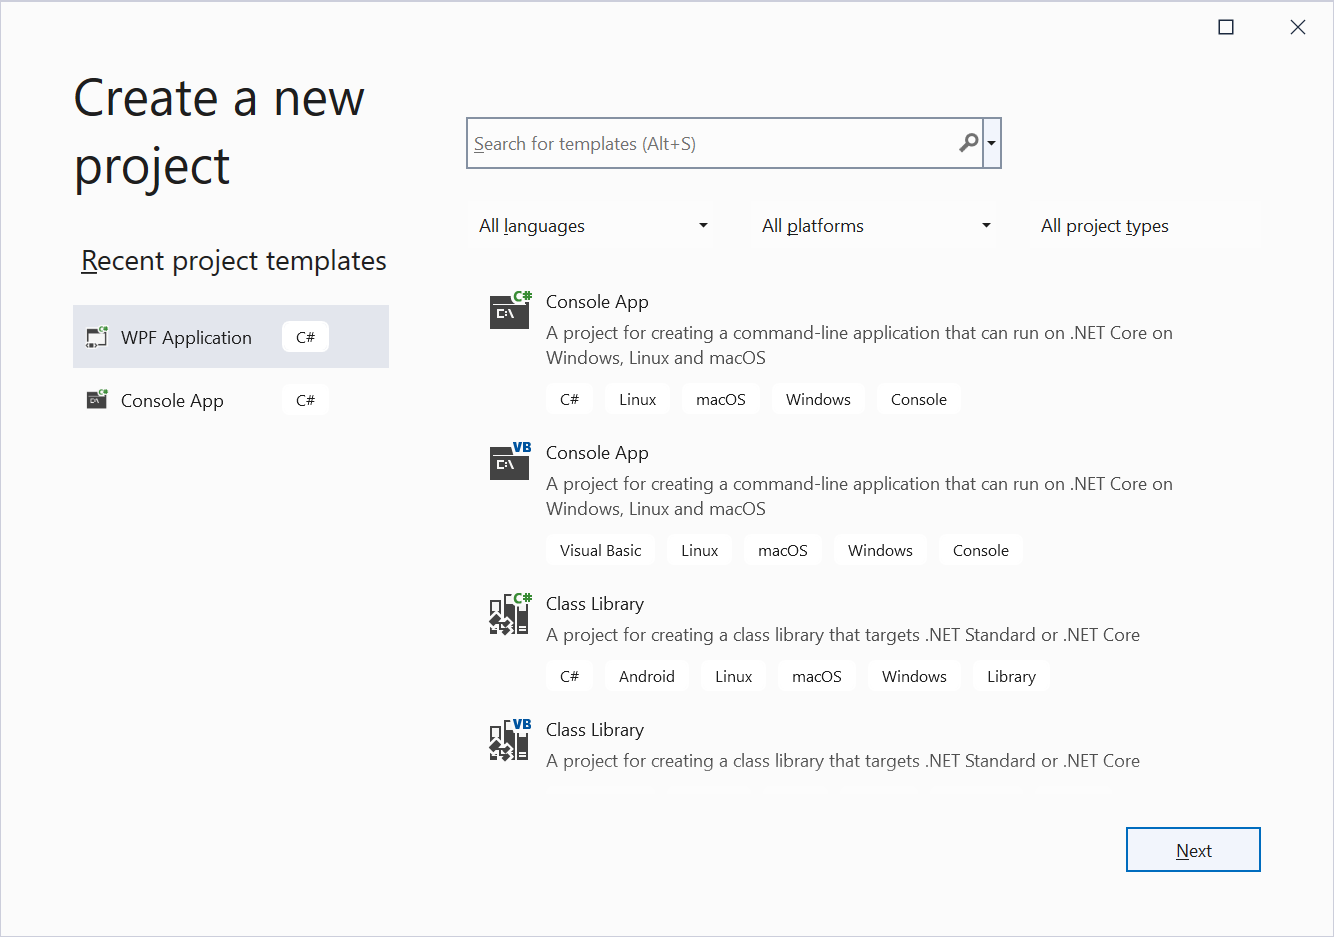
\includegraphics[scale=0.5]{CreateProject}

If you do not, click the "File" button at the top-left and choose "New->Project...".

When you get there, click "Console App", and name it with the appropriate chapter number. In the "Additional Information" section, make sure the "Do not use top-level statements" checkbox is checked.

When it starts, you'll need to type the code between the curly brackets after "Main" unless otherwise specified. You can run your program by clicking the green "Start" button in the toolbar, but note that in this chapter we won't make anything that will actually affect what is displayed when you press the button.

\section{Creating a variable}
Variables are created by first specifying the type of value they hold, the name that will be used to access the value at the variable, and finally what the variable equals.
Here is syntax to create a whole number variable. “Syntax” refers to how things must be written in order to be correctly processed by the computer:
\begin{CSharp}
int number;
\end{CSharp}
In the first section, we indicate the type of the variable; we  want it to store a whole number. This is why we write “int”, this is short for “integer”. Then, we create the variable itself: a concept known as variable declaration"\index{variable declaration}

We can then assign it a value like this:

\begin{CSharp}
number = 5;
\end{CSharp}
Note that the variable name appears to the left of the equals sign. Writing it as

\begin{CSharp}
5 = num;
\end{CSharp}
is invalid C\# code.
Oftentimes we'll know the value of a variable right when we are declaring it. We can make and give a value to a variable on one line:

\begin{CSharp}
int num = 5;
\end{CSharp}
\begin{CSharp}
int number = 5;
int numberCopy = number;
\end{CSharp}
\index{initialization}
Assigning a value to a variable is called \emph{initialization}, so when we create a variable and give it a value, we are both declaring and initializing a variable. 
Here are some variable name restrictions\index{variable name restrictions}:
\begin{itemize}
\item They have to start with a letter or `\_'
\item They can’t have any non-letter or non-number character (except underscores)
\item Spaces are not allowed
\end{itemize}

There are more than 70 keywords that cannot be used for variable names, which are listed \href{https://docs.microsoft.com/en-us/dotnet/csharp/language-reference/keywords/}{here.}

\section{Data Types}
Here are some of the basic data types\index{data types}, as well as what values they can hold.
\index{int}
\index{double}
\index{decimal}
\index{bool}
\index{char}
\index{string}
\begin{adjustbox}{max width = 15cm}
\begin {tabular} { l | c }
\hline

\textbf{Data Types} & \textbf{What They Can Hold} \\
\hline
   int & Whole numbers \\
   double & Numbers with decimal points \\
   decimal & Can hold double values, but is more precise. Better for financial calculations \\
   bool & Can hold true or false \\
   char & Holds text. Can only contain one text item. \\
   string & Can hold a series of chars. This is useful if you need to hold more than one character (e.g. words, sentences, etc). \\
   
\hline
\end{tabular}
\end{adjustbox}
\exercise
Identify what the best data type would be for each given data.
\begin{itemize}
    \item A person's name
    \item A person's ZIP code
    \item An abbreviation for a person's gender
    \item An identifier for whether or not a user is subscribed to a mailing list
    \item The amount of money in a bank account
\end{itemize}
Create variables for each of the above examples.
\exercise
See what happens if you try to give a variable a value that does not match its type (for example, attempting to use an integer value for a string).

\section{Writing char and string values}
 We need to add extra information when we are creating char and string variables. For chars, its value must be enclosed in single quotes. For strings, double quotes are used. Here are some examples:
\begin{CSharp}
char letter = 'a';
 
string word = "This is a string.";
\end{CSharp}


\section{Variable Computations}

You can also perform mathematical computations with variables. Here's how you can add two numbers, where x and y are initialized to 5 and 7 respectively:

\begin{CSharp}
int z = x + y;
\end{CSharp}
In this case, z would have the integer value of 12. You can also overwrite a variable with a new value:
\begin{CSharp}
int x = 5;
int y = 6;
x = y;
\end{CSharp}
\exercise
What are the values of x and y at the end of the code sample above?

\rule{\textwidth}{0.4pt}
\index{+=} \index{-=}
There are also the += and -= operators, which add or subtracts the value on the right side from the variable on the left, respectively. Given variable x:

\begin{CSharp}
x = x + 5;
\end{CSharp}
and
\begin{CSharp}
x += 5;
\end{CSharp}
are equivalent. However, the second one more directly expresses the intent of adding to the x variable.

\section{Comments}
\index{comments}
Let’s take a quick detour and discuss one of the simplest C\# aspects: comments. These are notes that programmers can leave in their application; they do not affect how the program runs. They are merely used by programmers to give themselves information on the intent of code. There are two types of comments:
\index{Single-Line comments|see{comments}}
\textbf{Single-Line Comments} These are only on a single line of code. A comment used in this fashion is preceded by two forward slashes. Here is an example:

\begin{CSharp}
//Declares an integer variable number and initializes its value to 5
int number = 5;
\end{CSharp}
Note that it is not recommended to use comments on such basic statements. They are more often used on more complex sections of code where it can be difficult to understand what is occurring; this instance is merely an illustrative example of implementing single-line comments.
\index{Multi-Line comments|see{comments}}
\textbf{Multi-Line Comments} These have starting and closing brackets that define when a comment begins or ends; they start with /* and end with */. Everything between these is processed as a comment.

Here is an example:
\begin{CSharp}
/*
Programmed by Alexander Summers
Creates integer variables and sets their values.
*/
 int x = 7;
 int y = 3;
 int z = 2; 
\end{CSharp}

\exercise
Suppose you were to create two string variables that are equal to “11.5” and “3.8.” If you were to add them together into a new string variable, what would that equal?
\exercise
What is the largest number an int can store? Hint: Look on 
\url{https://docs.microsoft.com/en-us/dotnet/csharp/language-reference/builtin-types/integral-numeric-types}
to answer this. Being able to read programming language documentation is important in the programming field.

\exercise
This sequence of statements is meant to set values to variables x, y, and z. What's wrong with it? 
\begin{CSharp}
/*
Creates integer variables and sets them to different values.
int x = 7;
int y = 3;
int z = 2;
\end{CSharp}

\section*{Going from Here}
The next two chapters will concern the principles and basic applications of methods and classes and how they interact with variables, which is important for using several of the special features built-in to the language. This will help us when we cover C\#'s application of the other core computer science aspects outlined in Chapter 1.
\chapter{Using Static Classes}
\minitoc

\section{Background Information: What are classes?}
Most programming languages allow programmers to access premade code, which allows programmers to write programs relatively faster as they don't have to stress some of the details. Microsoft has a vast set of features that are together called
\emph{.NET}, which include features that streamline everything from outputting to a computer console to creating modern graphical applications.

We can access elements of .NET through
classes\index{.NET!classes}, which group together related functionality. Programming, especially in C\#, involves either using classes that have already been made or creating our own. We'll learn about the latter part in a separate chapter; we'll just focus on what we've been given for now through .NET's classes.

\section{Introduction to the Console Class}
\index{Console class}
We will begin by learning about the
Console class. This allows us to make text-based applications; if you have worked with a command prompt in Windows, you have an idea of what our programs will look like. Console’s features can be accessed by typing “Console” followed by a period. You can think of the period as a way to access aspects of a class.

One of Console’s features (called methods in C\#) allows you to display string variables to the screen. This is called “Console.WriteLine(string);” Here is how you might use this in a program:
\begin{CSharp}
static void Main(string[] args)
{
    string introduction = "Hello world!";
    Console.WriteLine(introduction);        
}
\end{CSharp}
This program begins by creating a string variable that includes introductory text. The text enclosed in parentheses for our initial description of Console.WriteLine indicate an argument – this is what the programmer needs to supply in order for the method to work. We see that the method requires a string, so we supply it with “introduction”. 
Click the run button in the Visual Studio IDE to run the program. It looks like this: 
When you start your program, you should see something like this:

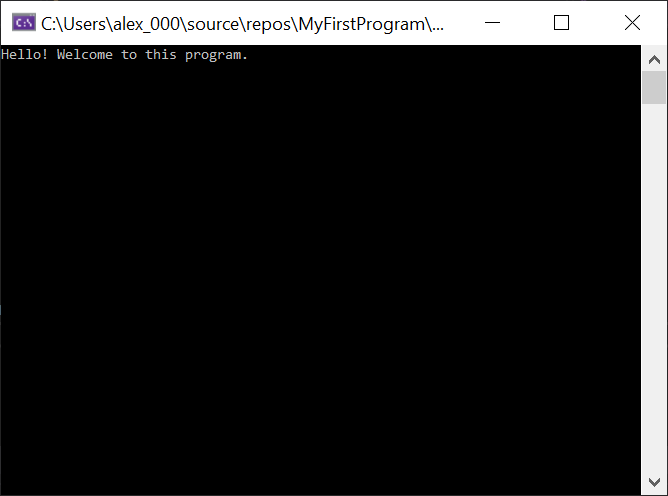
\includegraphics[scale = 0.5]{BasicHelloWorld}

Hooray! You’ve just created your first program that displays something to the user.
\section{Reading documentation}
How might you find out on your own how to use Console.WriteLine(string)? Let's take a quick detour through documentation on this topic; when we are programming professionally, we oftentimes need to reference information about a programming language and the libraries it has access to. Console.WriteLine() is provided by .NET, so let's look through the \index{.NET!documentation of}.NET documentation!

First, let's go to docs.microsoft.com.

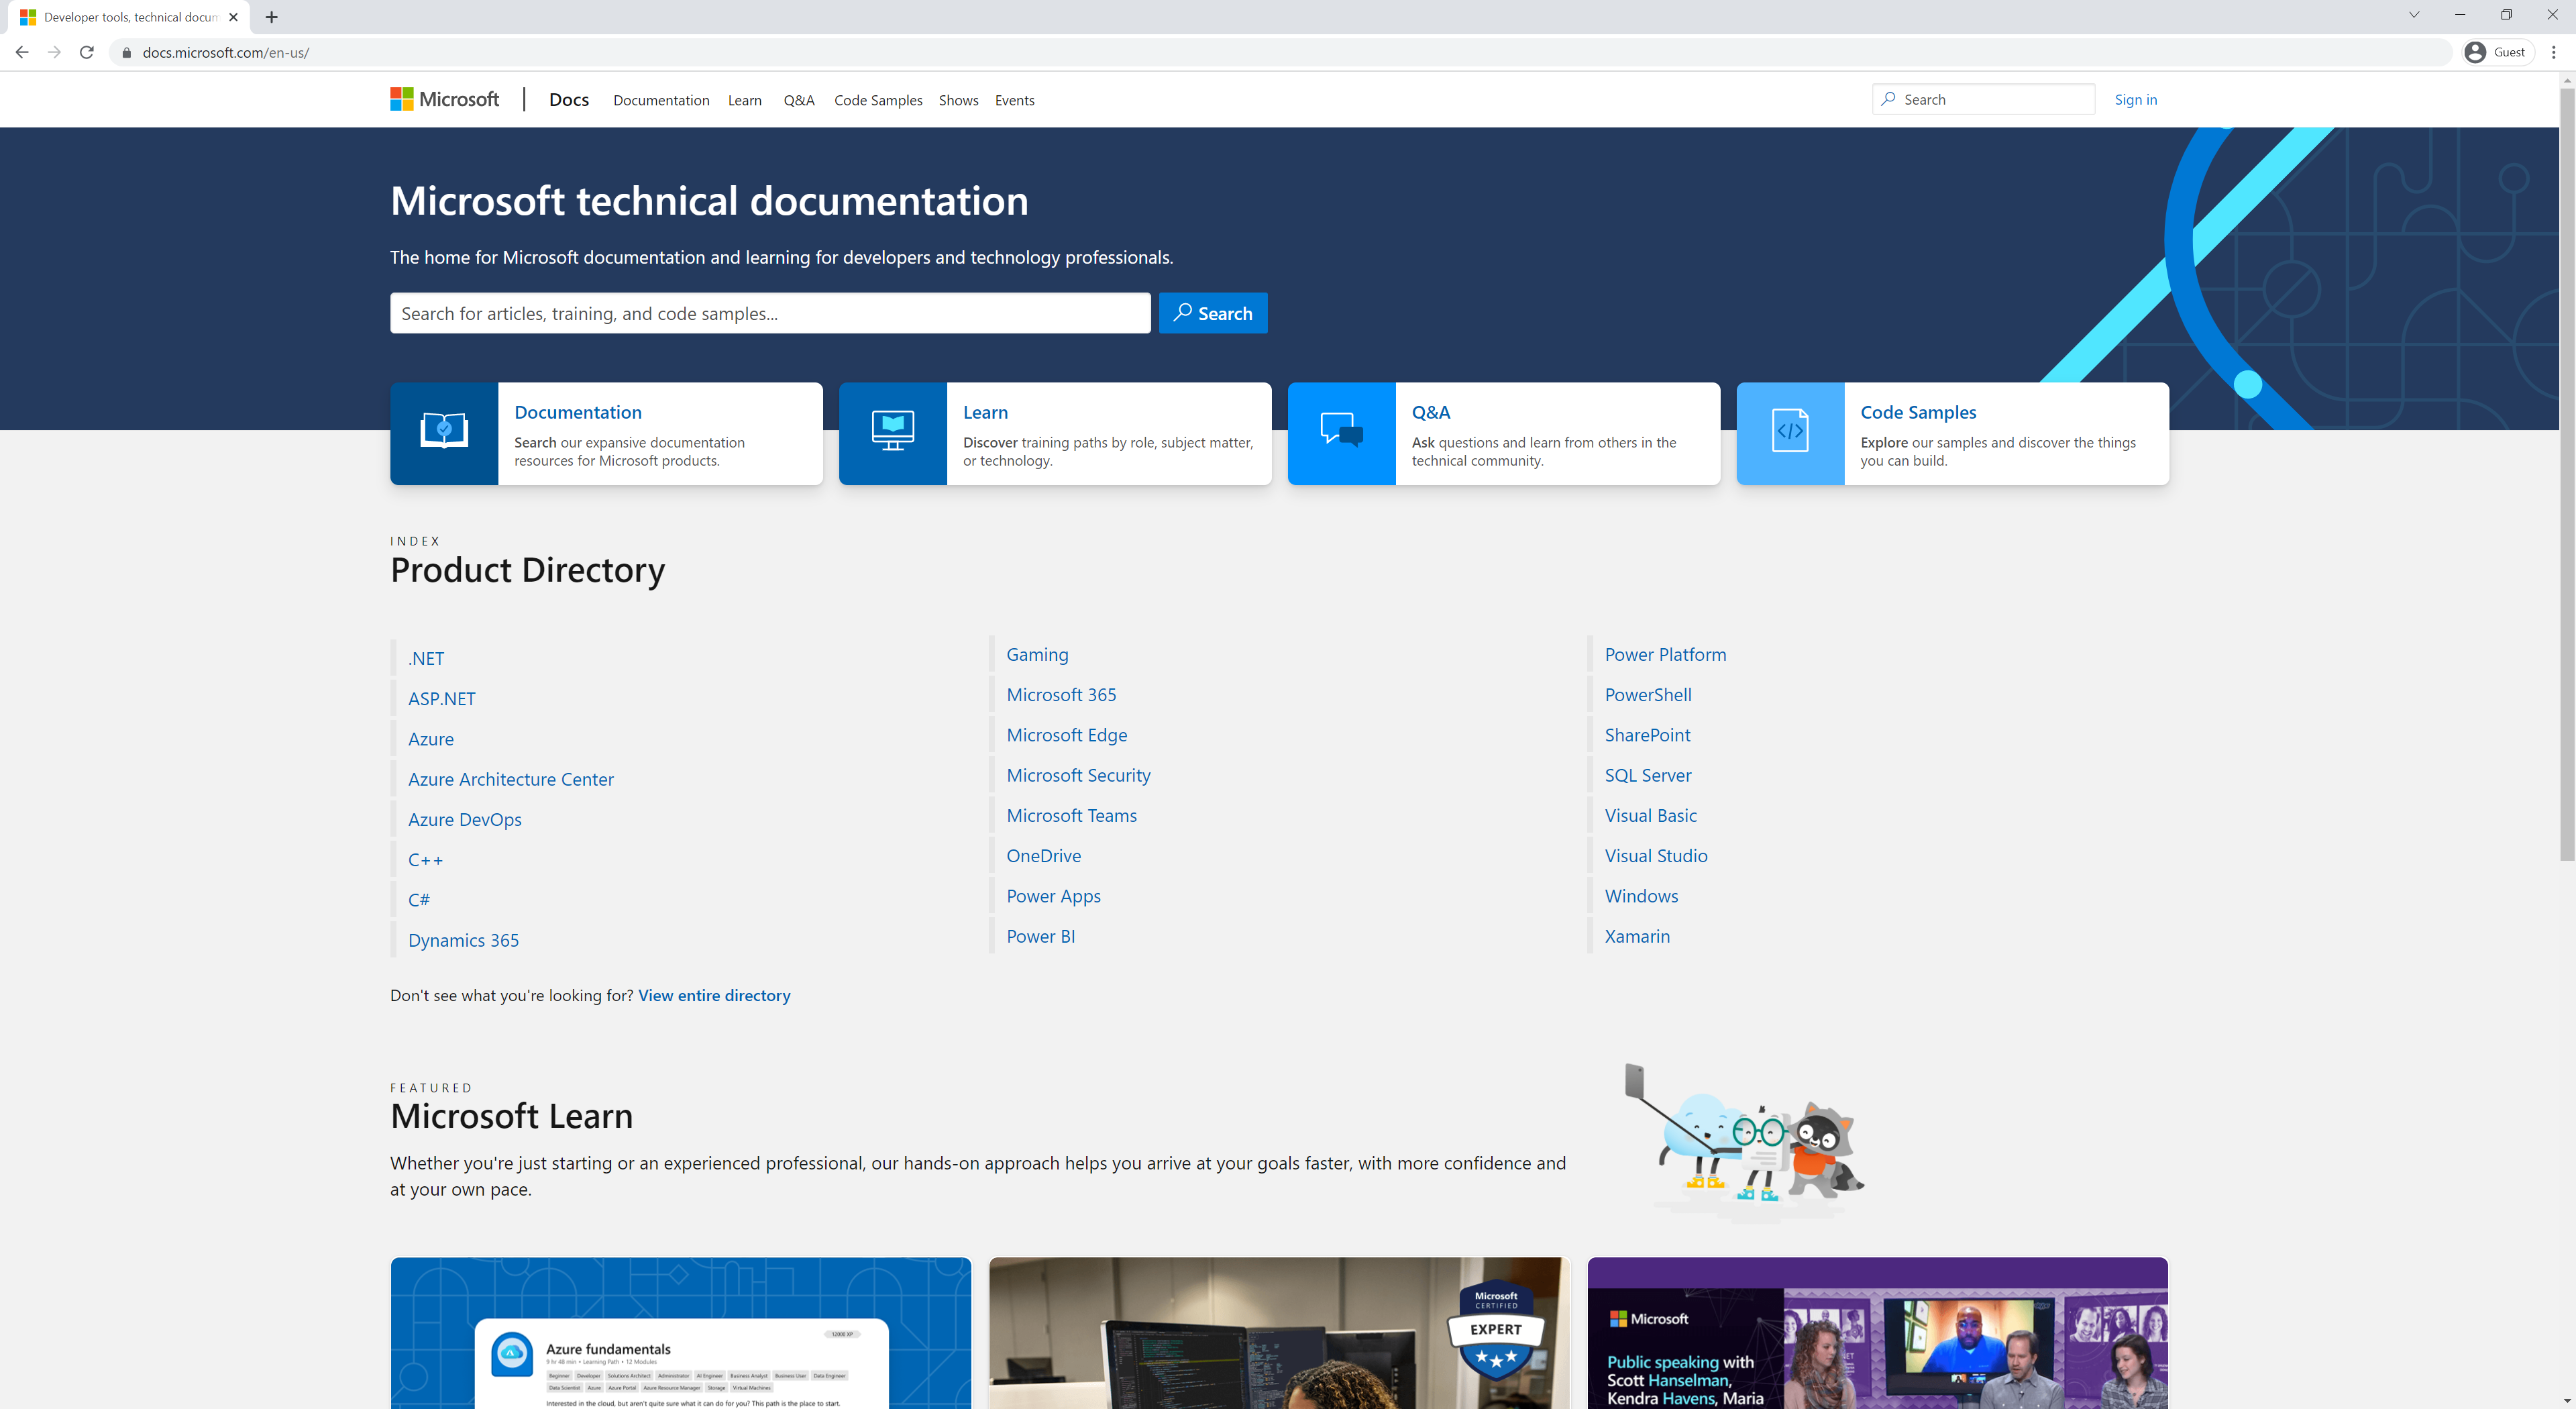
\includegraphics[scale = 0.2]{MicrosoftDocs1}

Then, let's click .NET in the docs directory section. You'll see this page:
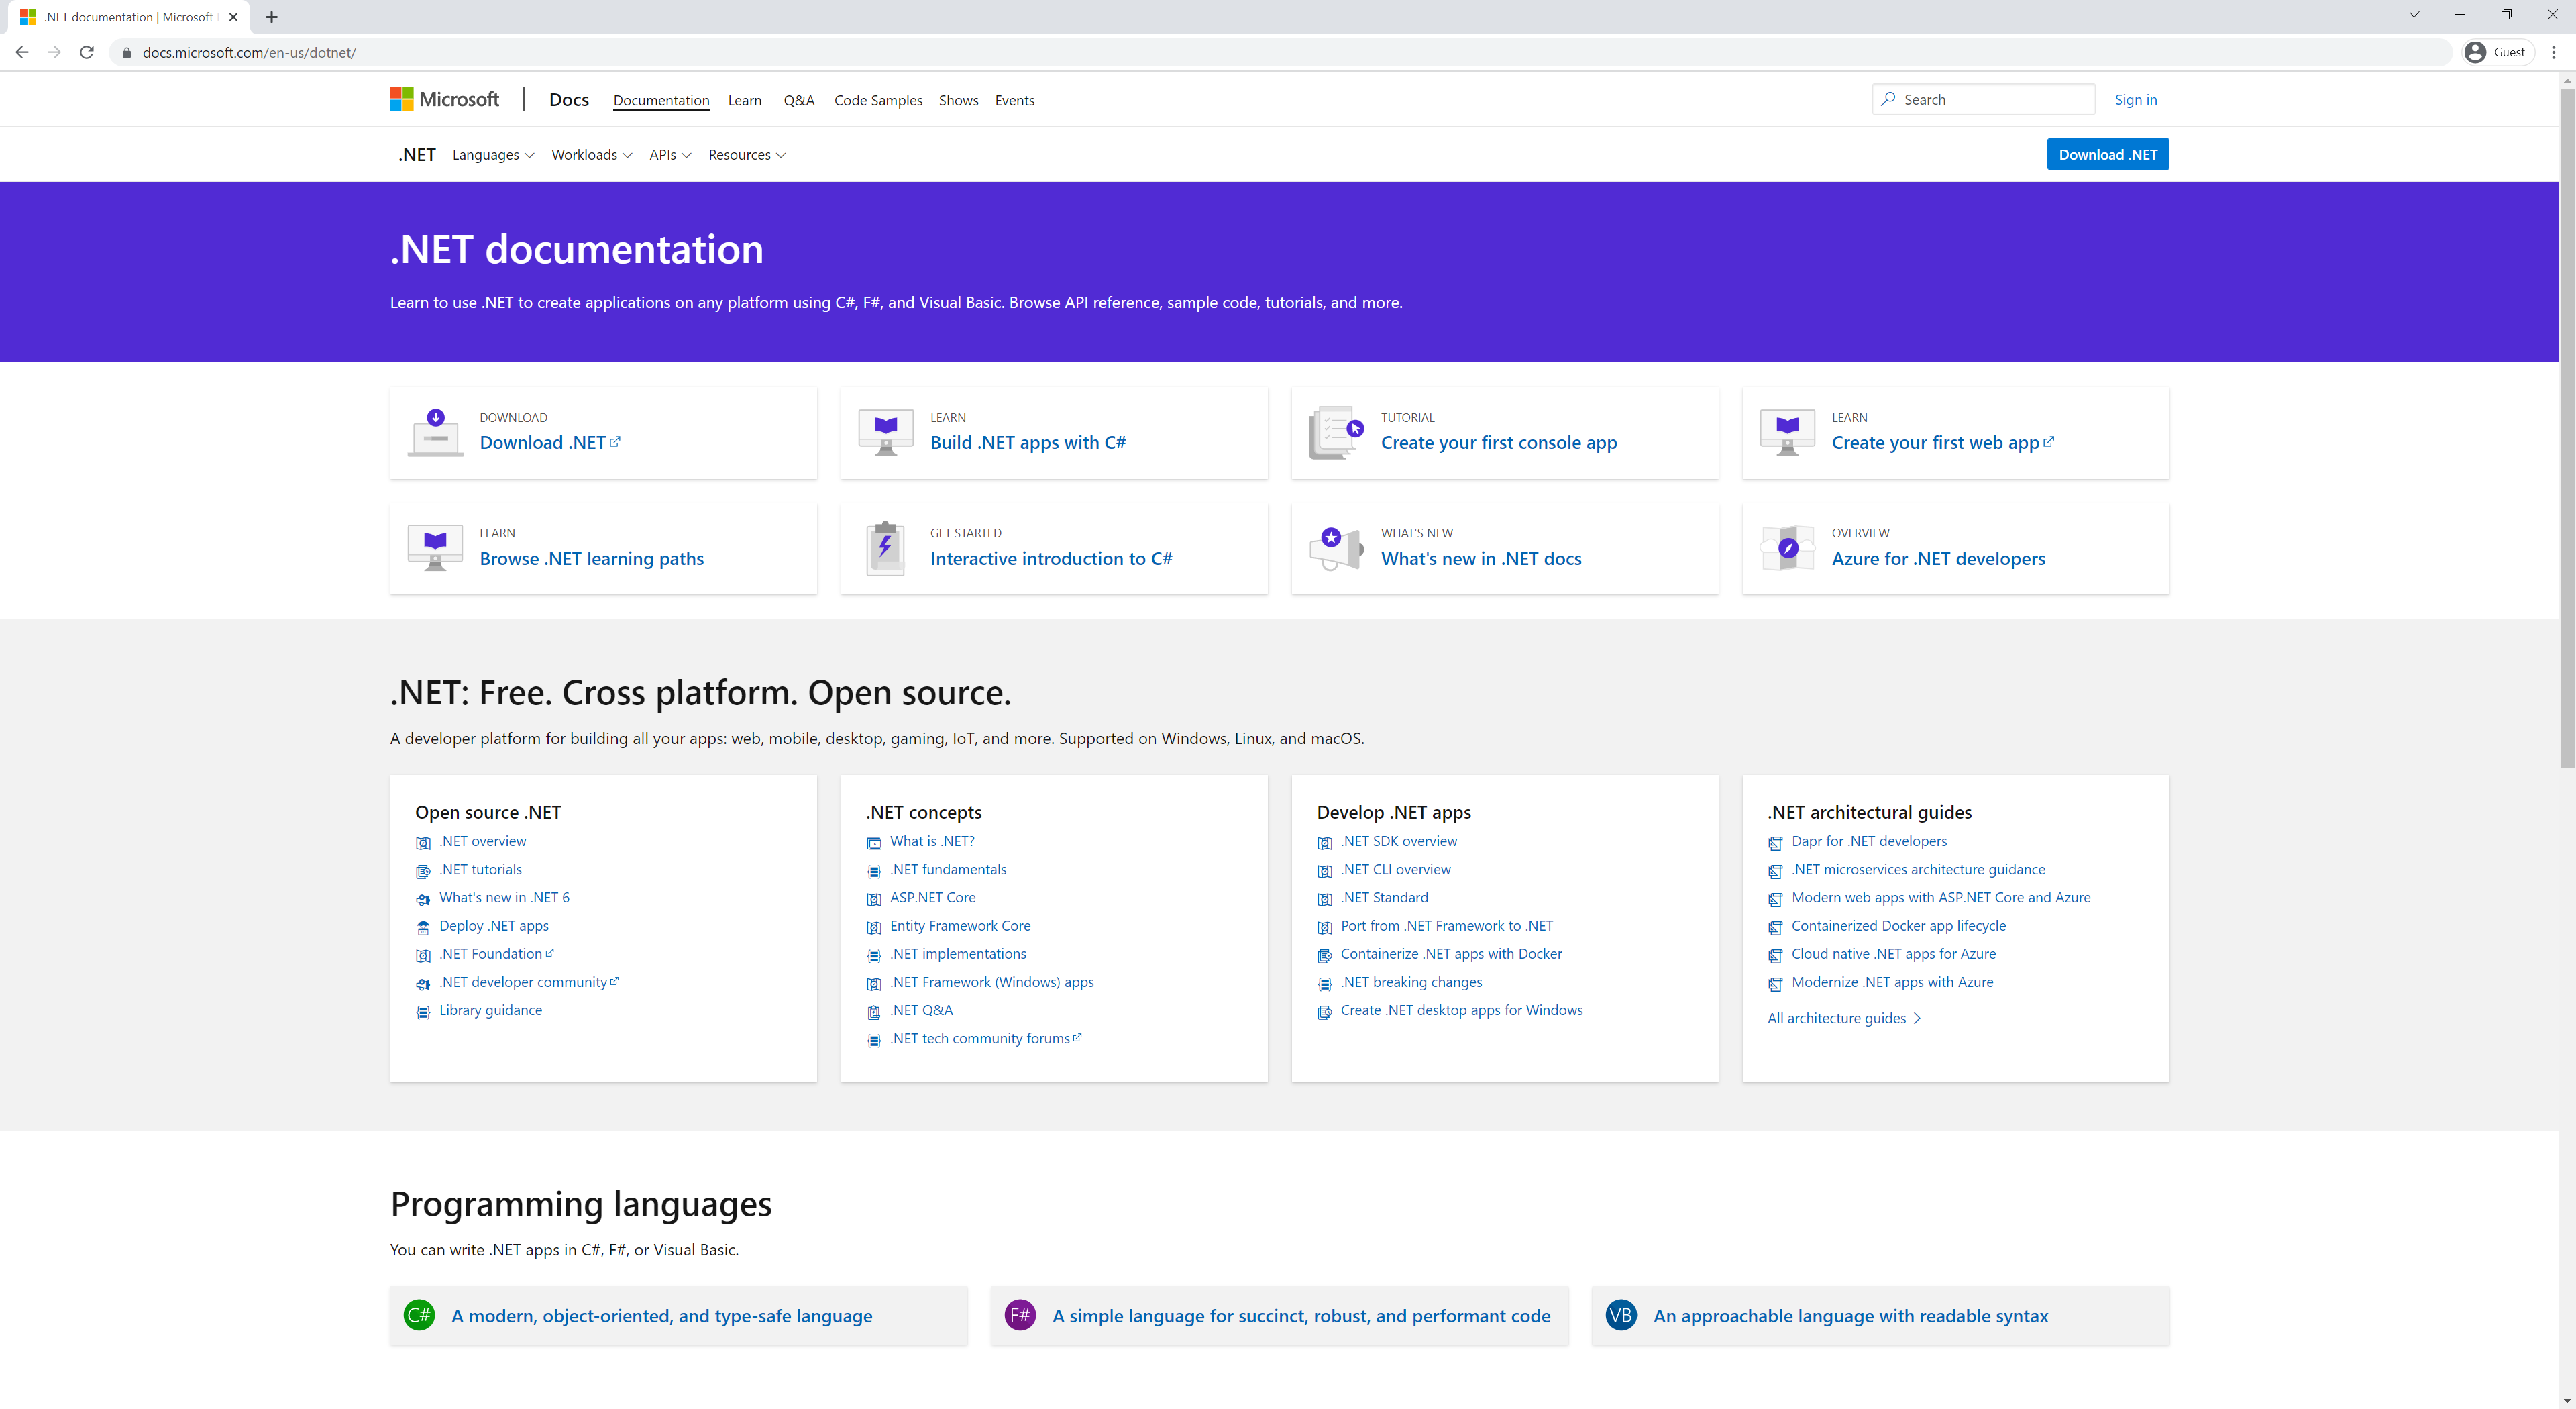
\includegraphics[scale = 0.2]{MicrosoftDocs2}
Then, you can type \index{Console.WriteLine} in the top-right search box.
\par\noindent\rule{\textwidth}{0.4pt}
There is another way we can write the above program. Instead of creating a variable to hold the introduction and then passing it through to WriteLine, we can directly insert the string as an argument. It looks like this:
\begin{CSharp}
Console.WriteLine("Hello! Welcome to this program.");
\end{CSharp}
There is a tradeoff for both strategies. If you want the data to be accessed or changed in the future, it is better to create a variable and include that in the method. If you directly include what the method requires, you cannot access that information later; you'll have to type out the information again.
\section{Processing User-Inputted Data}
Now, let’s mention allowing users to type in \index{user-inputted data} data into the program (otherwise known as user input). The user will be able to type in text, and it will be processed by the program. For this, we will use Console.ReadLine();
\begin{CSharp}
Console.Write("Please enter in your name: ");
string name = Console.ReadLine();
\end{CSharp}
Read the second line from right to left. First, the program will read a line from the console window, then it will take this information and insert it into the string “name”.
We can display it like this:
\begin{CSharp}
Console.WriteLine(name);
\end{CSharp}
\exercise
Change your program to exclusively use Console.WriteLine instead of Console.Write. How are the results different? Justify your answer by referencing the documentation, being sure to explain what a "current line terminator" is.

\rule{\textwidth}{0.4pt}
We can do more with output. The next section will concern writing to the screen (or printing) a combination of user strings and predefined ones.
\subsection{String Interpolation}

\index{string interpolation} String interpolation allows us to combine both variables and string literals into the same WriteLine method. We start by placing a \$ sign at the beginning of the WriteLine argument and continue with double quotes:
Console.WriteLine(\$"");
For predefined text, we type it in as normal. For variables, we enclose them in brackets:
\begin{CSharp}
string name = Console.ReadLine();
Console.WriteLine($"Hello, {name}!");
\end{CSharp}

\subsection{Converting User Input}
\index{converting user input} We can also convert user input so we can process it in a proper fashion. For example, we can’t process user input as a number immediately, as Console.ReadLine considers text input to be a string. We need to convert it to an integer before we can perform mathematical operations on it. We can use the Convert class for this:
\begin{CSharp}
Console.WriteLine("Please enter in a string.");
string numberAsString = Console.ReadLine();
int number = Convert.ToInt32(numberAsString);

int numberPlusFive = number + 5;
Console.WriteLine($"Your number plus five is: {numberPlusFive}!");$
\end{CSharp}
Convert.ToInt32 accepts a string as an argument. It then converts it to an integer and sets it as the value of an integer variable named “number”. With this, we can perform mathematical computations on our value, as mentioned in Chapter 2.

An equivalent if we want to convert a string to a double value is Convert.ToDouble. For example:

\begin{CSharp}
string numberAsString = Console.ReadLine();
double fahrenheit = Convert.ToDouble(numberAsString);

double celsius = fahrenheit - 32 * 5 / 9;

Console.WriteLine(celsius);

\end{CSharp}
Note that WriteLine can process more than strings. It can handle other variable types, such as integers and doubles, as shown in the above examples.

\exercise
Write a program that prompts the user to enter in a number with decimals. Convert it to a double and add 7.5 to it. Assume the user will actually input a number and not something else (e.g. a word). Print the new value to your display.

\exercise
Write a program that prompts the user to enter in two integers. Create variables for the sum, difference, product (use *), quotient (/) and remainder (\%) between the numbers. Add up all of these values into an integer variable and output it with Console.WriteLine. 

\exercise
You may have noticed that the quotient from Exercise 3-3 displays the value as a whole number. Why is that? How could you change it to display it with decimals?
\exercise
Create a program that accepts a number, calculates the whole number and decimal portions of the number, and outputs both on separate lines. Solving the decimal portion will require some thought about potential usage of the operators defined in Exercise 3-3.
\chapter{Creating Methods}
\minitoc
\section{What are Methods?}

Methods allow you to enclose program statements that can be called in other locations, whether they be in the same file or not. When they are invoked (or called) within the programmer’s code, the contents of the method are run just as if we were to include those details directly in our Main method.

We have worked with methods including WriteLine and ReadLine, which are located in the Console class. When we used those in our code, our computer went to the Console class (which is located in a hidden file) and performed the statements that are located in their respective methods.

\section{Making Methods}
To create a method in a console program, the word “static” should be used at the beginning. This allows it to run without needing to create an instance of our program class. Since we're simply going to utilize the method in this file, using "static" simplifies our work.
The next step is to declare a return type. This is the value the method gives back to what called it. Methods can return any data type. If we do not want to return anything, we use the “void” keyword. 

Then, we must give a name to the method to identify it in our program.

Afterward, we supply parameters into the method to process; this is enclosed within parentheses after the name is declared.
Then, we place left and right curly braces, where we put the contents of our method.
Let’s make a method now.

\section*{Example 1}
Our first method will be simple. When it is called, it will display a predefined message to the screen.
Here is how we would first create the method (remember to create it outside of Main, but within the brackets of the Program class):
\begin{CSharp}
static void DisplayMessage()
{
       
} 
\end{CSharp}

Then, we will write the necessary code inside of the method. We do not need to write much:

\begin{CSharp}
static void DisplayMessage()
{
    Console.WriteLine("Hello!");
}
\end{CSharp}

Now we will call this inside of Main:

\begin{CSharp}
static void Main(string[] args)
{
    DisplayMessage();
}
static void DisplayMessage()
 {
   Console.WriteLine("Hello!");
 }
 \end{CSharp}
 
 Inside the Main method, the first (and only) line of code calls DisplayMethod. The program transfers from Main to DisplayMethod and runs the code there. 
 
 
 \begin{figure}
     \centering
     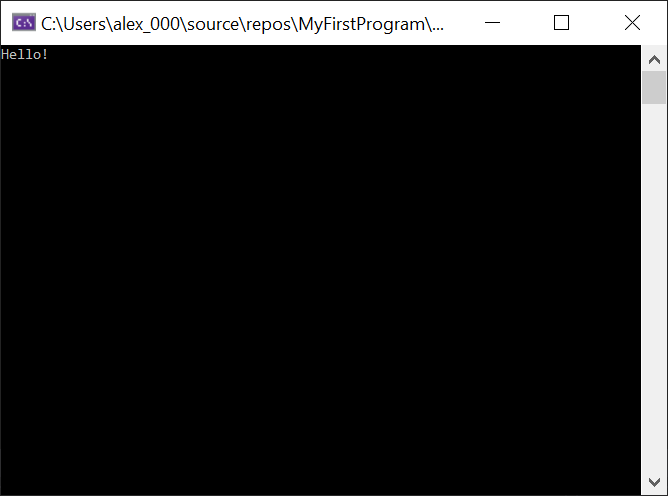
\includegraphics[scale = 0.5]{MethodHelloWorld}
     \caption{This will display (or output) ``Hello!'':}
     \label{fig:my_label}
 \end{figure}
 If we wanted greater customizability, we would have a string parameter that will be processed in the method:
 
 \begin{CSharp}
 static void DisplayMessage(string messageToDisplay)  
{  
/* The contents in parentheses represent an argument; 
    when using the method a string must be supplied */
    Console.WriteLine(messageToDisplay);
}
\end{CSharp}
The variable name is an indicator when we're using the method for what we should use as an argument. The parameter name itself has no bearing on the name of the variable that you call the method with.
\exercise
Test out your method. Try calling it in Main and giving it different values (such as a string variable and directly typing in a string). Then, run the program.

\exercise
Methods can be defined with more than one parameter which must be separated by commas. On docs.microsoft.com, research the Console.ForegroundColor property. Add a parameter to DisplayMessage that accepts a color and sets the foreground color to that. 

\exercise

Expand your calculator program from Exercise 2-2. Create a method that stores the calculator program and call it inside Main.

\exercise
Implement your code from Exercise 1-3 as a C\# method.

\section{Returning Values}

In our previous programs, we wrote void as our return value; this means that our methods returned nothing. Control passed from Main into our method, but never brought any values back to our Main method. As stated before, methods can return values. Such examples include integers, strings, and any other data type.  
Here is a simple program that takes two strings and combines them in a more formal \emph{lastname, firstname} format:
\begin{CSharp}
 static string CreateName(string firstName, string lastName)
{
    string name = lastName ", " + firstName;
    return name;
}

\end{CSharp}
Methods process statements line-by-line until a return statement is reached; the program then continues in the method where it was called. Please note this is true even of void methods -- the return statement is implied and doesn't need to be written.
Return statements allow methods to be used in place of variable information. Here are some examples with string variables:

\begin{CSharp}

string fullName = CreateName("Donna", "Noble");

Console.WriteLine($"Hello, {CreateName("Frank", "Reynolds")}!");

\end{CSharp}

We created a "name" variable inside our CreateName method; why not use that directly in Main? The variable "name" is only available within the method it is declared; Main doesn't have access to it. Therefore, CreateName passes the value of "name" to our Main method and sets it to a variable inside it so we can use it there.

\exercise
What happens if you set the double value that the calculator returns as the value of an int variable in the Main method?
\exercise
Using your knowledge so far, give a basic description concerning how Console.ReadLine(); works.


\rule{\textwidth}{0.4pt}
Methods are useful because they allow you to organize your code into distinct units based the completion of particular tasks. For example, we might write a program that, over the course of its run, prompts the user for values and uses them to displays some result. In the method that checks for user input, we are not specifically concerned about how the values are processed: just that it returns a correct. We can create a method to process these values so that when we are looking at our code later we can simply read the basic user input code, and, if we care about the details of how the values are processed, we can look at that particular method.
\exercise
Write a method that accepts various values and displays the results of a Mad Libs game. You can define the template for the Mad Lib in your method, as well as any parameters.

Here's how you might call the method, supposing that you prompted the user for values earlier on:
\begin{CSharp}
Console.WriteLine(madLib("cat", "green", "silly");

//This might output:
//The cat sat on the green man who was very silly.
\end{CSharp}
After the value is outputted for the first time, prompt the user to enter in values once more.
\exercise
Write a method that accepts an integer argument. Have the method calculate and return the negation of that number. For example, supplying an argument of 5 would return -5, while an argument of -3 would return 3.
\exercise
Write a method that calculates the slope of given coordinates $x_1$, $y_1$ and $x_2$, $y_2$. That is, given the aforementioned coordinates, return a value that is equal to
\[
\frac{y_2 - y_1}{x_2 - x_1}
\]
Then, write a program that asks the user to enter in values. Prompt them and allow them to enter in a value three times.
\exercise
Write a method that calculates one of the roots of a quadratic equation. It should take three doubles corresponding to values \emph{a}, \emph{b}, and \emph{c} and output a value equal to

\[
\frac{-b \pm \sqrt{b^2 -4ac}}{2a}
\]
Then, write a program based on this method that asks the user to enter in values. Prompt them and allow them to enter in a value three times.
You can use the built-in Math.Sqrt method to calculate the square root of a given number, and the Math.Pow method to compute the value of a number to a given exponent.


The sign that looks like a plus on top of a minus means, "plus or minus," which indicates there are two possible values of the formula given the three values: where that sign is read as a plus or as a minus. In this case, you can choose to interpret the sign as either of those two. Later, we will learn how we can return both of those values.


These two aspects allow your Main method (and methods that call other methods) to be more concise and readable, because the code to complete particular tasks are partitioned into their own methods. 
\section{Variable Scoping}
Suppose we had a variable in a method:
\begin{CSharp}
static void setValue(int num)
{
  int numberToSet = num; 
}
\end{CSharp}

and we wanted to access the variable outside of the method. Perhaps, for example, we want to use Console.WriteLine() to display our number. If we try to do this, we get an error:

\begin{verbatim}
    CS013: The name 'numberToSet' does not exist in the current context
\end{verbatim}
This issue delves into the idea of \emph{variable scope}. We are obtaining this error because we declared the variable \emph{numberToSet} within the setValue method. The sections of code outside of that method do not know that variable exists.

If we would have declared our variable outside of \emph{setValue}, we would be able to access it both outside and inside the method:

\begin{CSharp}
int numberToSet;
setValue(8);
static void setValue(int num)
{
  numberToSet = num; 
}
\end{CSharp}

The general idea is that variables declared in a section of code enclosed in brackets cannot be accessed in code sections outside of them. While it may seem convenient to declare all of our variables in the outermost section of our code, it is good practice to only declare them in the \emph{scope} that we expect it to be used. This will prevent accidental use of a variable in contexts where we do not actually want them to be accessible, and make it clearer to readers of our code how our variables fit in to our program.
\exercise
The below code examples declare and attempt to display the value of a variable. Describe in each example whether use of \emph{Console.WriteLine()} will work as expected or cause an error.
\subsection*{1.}
\begin{CSharp}
int num;
setValue();
static void setValue()
{
    num = 5;
}
Console.WriteLine(num);
\end{CSharp}
\subsection*{2.}
\begin{CSharp}
setValue();
static void setValue()
{
    int num = 5;
}
Console.WriteLine(num);
\end{CSharp}
\subsection*{3.}
\begin{CSharp}
setValue();
int num = 3;
static void setValue()
{
int num = 7;
}
Console.WriteLine(num);
\end{CSharp}
\section*{Going from Here}
In the next chapter we'll cover the use of if statements and while loops, which we previewed in Chapter 1! We'll also cover the do-while loop: it's similar to the while loop, except it is used in circumstances where we want a block of code to run at least once.
\chapter{Booleans \& Decision Structures}
\minitoc
\section{What are Booleans?}
\index{true}
\index{false}
Boolean values consist of either “true” or “false”. They are used to evaluate the truthfulness of statements. Here is an example:
\begin{CSharp}
int x = 3;
int y = 3;
bool isEqual = (x == y);


\end{CSharp}
\index{==}
In this statement, the validity of whether x equals y is checked. The equality operator (==) checks if two values are equal. Since x and y both hold the values of 3, isEqual is set to “true”.

\index{!=}
There is also the inequality operator (!=). As the name implies, it checks whether two or more values are not equal to each other:
\begin{CSharp}
int x = 3;
int y = 5;
bool isEqual = (x != y);
\end{CSharp}
In this case, isEqual would be true; x is not equal to y.
\index{if}
Booleans can be checked to determine whether code should be run or not with if-statements. For example:

\begin{CSharp}
int x = 9;

if (x > 7)
{
    Console.WriteLine("x is greater than 7!");
}
\end{CSharp}
\index{else-if}
We can use else-if to check for other conditions:

\begin{CSharp}
int x = 9;

if (x > 7)
{
    Console.WriteLine("x is greater than 7!");
}
else if (x < 7)
{
	Console.WriteLine("x is less than than 7!");
}
\end{CSharp}
\index{else}
We can use else without adding an if as a catch-all; if the statement in if blocks are not executed, execute the contents in else:
\begin{CSharp}
int x = 9;

if (x > 7)
{
    Console.WriteLine("x is greater than 7!");
}
else if (x < 7)
{
	Console.WriteLine("x is less than than 7!");
}
else
{
	Console.WriteLine("x is equal to 7!");
}
\end{CSharp}
Since x being greater than 7 is true, the code under (x>7) executes.

\exercise
\index{number-guessing game}
Create a basic number-guessing game. Accept user input and place the value in an integer variable. Then, compare it to an integer variable with the solution. If the user types in the correct number, write to the screen something to the effect of “You’ve won!” Try running the program – first input the correct answer, then re-run the program and try inputting an incorrect answer.
\index{String comparisons}
\index{Inches/Feet converter program}
\section{String Comparisons}
Just like we can compare integer and double variables, we can compare strings, too. Supposing we wanted to create a program that does a particular task based on user input:

\begin{CSharp}
Console.WriteLine("Welcome to the inches/feet converter.");
Console.WriteLine("Please enter in the number you want to convert.");

double numberToConvert = Convert.ToDouble(Console.WriteLine());

Console.WriteLine("Do you want to convert from inches to feet or feet to inches?");

string conversionChoice = Console.ReadLine();

double conversionResult;
if (conversionChoice == "feet to inches")
{
    conversionResult = numberToConvert * 12;
}
else if (conversionChoice == "inches to feet")
{
    conversionResult = numberToConvert / 12;
}

Console.WriteLine($"Your value is {conversionResult}");
\end{CSharp}

As you can see, string comparison is much like integer comparison. The principles of any sort of value comparison are the same.
There is one more important element, however, that we need to consider when we are comparing char or string values: such comparisons are \emph{case-sensitive}. The user needs to enter the words exactly as they are written (that is, without capitalization differences) in order for the corresponding if section to trigger.

Luckily, we can standardize the variable values that are being compared with by using char and string's ToLower() method. So, if the user would enter in, say, "Feet to inches", "fEEt tO Inches", or other variants, ToLower() would convert the value to "feet to inches", allowing the comparison to work as expected. Note that if the user inputted "feet to inches", the ToLower() method would effectively do nothing.

\begin{CSharp}
Console.WriteLine("Do you want to convert from inches to feet or feet to inches?");

string conversionChoice = Console.ReadLine().ToLower();

\end{CSharp}

\noindent\rule{12.5cm}{0.4pt}

\index{less than symbol (<)}
\index{greater than symbol (>)}
There are more operations that can be supported besides equality and inequality. You can also check whether one value is greater or lesser than the other (> or <), and you can check if a value is greater than or equal to another value or the reverse with >= and <=. 
You can also check Boolean values directly in if-statements.
\begin{CSharp}
bool value = true;

if (value == true)
{
    Console.WriteLine("This value is true!");
}
\end{CSharp}
Since “value” being equal to true is correct, Console.WriteLine prints a message.  
\exercise 
What would've happened if we would have written and ran this:  


\begin{CSharp}
bool value = true;

if (value == false)
{
    Console.WriteLine("This value is false!");
}
\end{CSharp}

\exercise
\index{absolute value exercise}
Create a method that programmers can use to obtain the absolute value of an inputted value. To be more specific, it will need two return statements: one that simply returns the argument if it is greater than or equal to 0, and another that negates the value otherwise.

\rule{\textwidth}{0.4pt}

Since if/else already resolves the information in its parentheses as Boolean (true or false) values, we do not need to explicitly declare whether a variable == true or == false. A more organized way to write such expressions, therefore, is:
\begin{CSharp}
bool value = true;

if (value)
{
 Console.WriteLine("This value is true!");
}
\end{CSharp}
\index{logical negation operator}
Another way to check if a Boolean value is false is the logical negation operator. It can be written as:
\begin{CSharp}
else if (!value)
{
    Console.WriteLine("This value is false!");
}
\end{CSharp}
\exercise
Describe the output of these two code samples:
\begin{CSharp}
bool value = true;

if (value)
{
  Console.WriteLine("true");
  value = false;
}
if (!value)
{
 Console.WriteLine("false");
}

\end{CSharp}
\begin{CSharp}
if (value)
{
  Console.WriteLine("true");
  value = false;
}
else if (!value)
{
 Console.WriteLine("false");
}
\end{CSharp}
\exercise 
Allow the user to input a number. If the number is greater than 10 AND less than 30, output the number.

\section{Int32.TryParse}
\index{Int32.TryParse}
Let’s look back at our earlier number-conversion program from chapter 3:  

\begin{CSharp}
Console.WriteLine("Please enter in a number: ");

string numberAsString = Console.ReadLine();
int number = Convert.ToInt32(numberAsString);

int numberPlusFive = number + 5;

Console.WriteLine($"Your number plus five equals: {numberPlusFive}");

\end{CSharp}

There is another strategy: TryParse. 
\index{Int32.TryParse!definition}
TryParse accommodates invalid input with its use of Booleans; if a value can be converted, the method returns true, as well as including the actual converted value. You can include code in an else section that runs when the value cannot be converted. So, you should use TryParse over Convert in the case of trying to convert user input that may not succeed; for example, in the case where a user inputs a sequence of letters when the program is expecting to convert input to an integer. Note that integers and doubles can always be converted to a string value, but string values are not always convertable to a numeric type.

Now, let’s solve our problem with TryParse:

\begin{CSharp}
Console.WriteLine("Please enter in a number: ");

    string numberAsString = Console.ReadLine();
            
if (Int32.TryParse(numberAsString, out int value)
{
        int numberPlusFive = value + 5;

        Console.WriteLine($"Your number plus five equals: {numberPlusFive}");
}
else
{
    Console.WriteLine("You did not type in a number.");
}
\end{CSharp}
\index{Int32.TryParse!out parameter}
Note the “out” used in Int32.TryParse. This allows us to use the variable "value" in our code, which has the value of the converted numberOfString. We do not need to know much about out parameters in this book: just that they allow methods to return multiple values (that is, additional values beyond a method's defined "return value").


\index{Boolean logical operators}
\section{Boolean Logical Operators}
Earlier, you were asked to print a number if it were within the bounds of two integers: 10 and 30. You may have solved it like this:  

\begin{CSharp}
static void Main(string[] args)
        {
            string numberAsString = Console.ReadLine();

            int number = Convert.ToInt32(numberAsString);

            if (number > 10)
            {
                if (number < 30)
                {
                    Console.WriteLine(number);
                }
                
            }
        }

\end{CSharp}
We are now going to go over an easier way to complete this, which gives us a nice introduction o Boolean logical operators.  
\index{\&\&}
In C\#, multiple conditions can be checked in an if statement. The conditional logical AND operator (\&\&) can be used to check if the expressions to the left and right of it are both true. 

Here is what our number-processing program would look like with an \&\& operator and our knowledge of Booleans:

\begin{CSharp}
static void Main(string[] args)
        {
            string numberAsString = Console.ReadLine();

            if (Int32.TryParse(numberAsString, out int number)
            {
                if ((number > 10) && (number < 30))
            {
                    Console.WriteLine(number);
            }
                 else
                 {
                        Console.WriteLine("Your number is not between 10 and 30.");}
                 }
            else
            {
                    Console.WriteLine("Your input is not a number.");)}
        }

\end{CSharp}
\index{||}
There is also the conditional logical OR operator (||). This checks if either the value to the left or to the right of it is true.

\exercise
Rewrite the above program so it prints the number if it is greater than 10 OR less than 30.

 
\exercise
Place our above program into a method that returns a Boolean and takes a user-inputted integer as an argument. If the number fulfills the criteria as stated before, return true – otherwise, return false.
\index{Choose Your Own Adventure exercise}
\exercise
For this exercise, create a basic Choose Your Own Adventure game that reads in user input and displays output based on what the user types; it does this until the player reaches an end point.   


\section{The While Loop}
\index{while}
While loops can be used to repeatedly run code while a condition is true. For example:  
\begin {CSharp}
bool booleanVariable = false;

while (!value)
{
    Console.WriteLine("booleanVariable is false!");
}


\end{CSharp}
\exercise
Using a while loop, print out the numbers between 1 and 1,000, inclusive.  
\exercise
Write a program that accepts input that is converted to an integer. If the value cannot be converted, ask for input again.

\section{The do-while Loop}
\index{do-while}
Sometimes we'll want to run code that would be great in a while loop, but it should be run once, regardless of the condition. This is where the do-while loop comes in handy. It runs the block of code, then checks the condition. If it is true, the block of code is run again.
\exercise
What does the below code do?

\begin{CSharp}
int solution = 50;

Console.WriteLine("Can you guess the number between 0 and 100?");
int guess;

do
{
    while (!Int32.TryParse(Console.ReadLine(), out guess))
    {
        Console.WriteLine("Your input is not a number.");
    }
    
    if (guess < solution)
    {
        Console.WriteLine("Your number is too low!");
    }
    else if (guess > solution)
    {
        Console.WriteLine("Your number is too high!");
    }
}
while (solution != guess);
             
Console.WriteLine("Done.");



\end{CSharp}
Note the semicolon after the parentheses in the while section; that is required (though it isn't with the normal while loops) 
\section{A Brief Detour into Debugging}
\index{debugging}
As our programs become ever more complex, it becomes increasingly likely that we will run into bugs, or errors, in our program. In these cases, it is often useful to step through our code line-by-line to follow the logic of our programs. Visual Studio, for its part, facilitates this by allowing us to stop execution of our program while it is running once it gets to a given point and allow us to view the current values of our variables.

For our example, copy the code from Exercise 5-14 into Visual Studio.

Suppose we wanted to stop our program at a specific line. The Visual Studio feature that allows us to do this are called "breakpoints".

Look at the code window. At the left of our line numbers, you'll see this dark-gray line:



\includegraphics[scale=0.2]{breakpointline}

If you double-click at a point, you'll set a\index{breakpoint} breakpoint at the particular line that your mouse is next to.

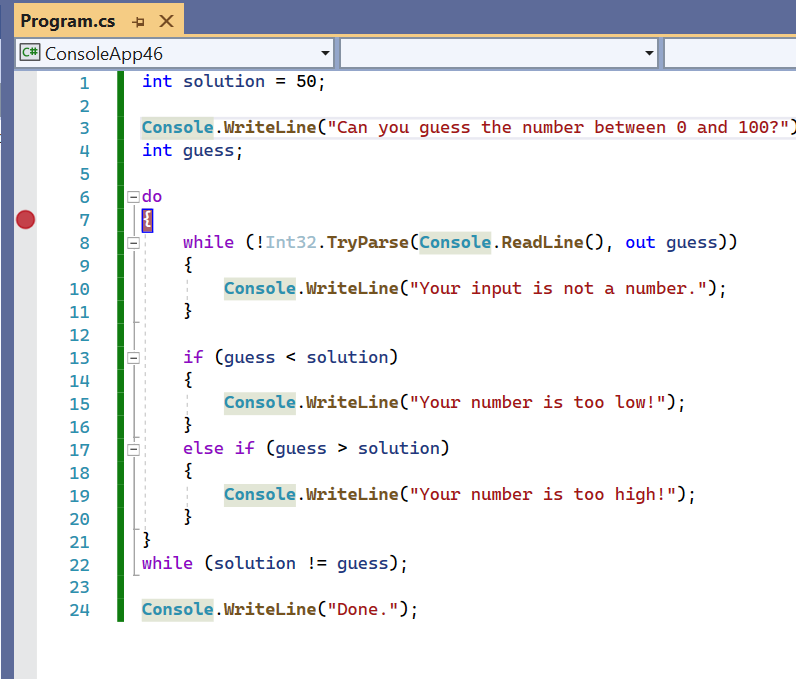
\includegraphics[scale=0.40]{breakpointset}

This indicates that we want to pause our program at that particular line: in this case, the beginning of the do loop.

If we run the program, we'll see that our program in fact stopped at the point we set.

Look at the bottom of the screen:

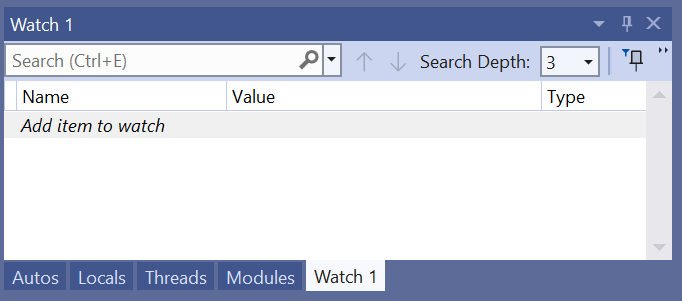
\includegraphics[scale=0.5]{watch}
Make sure the tab at the bottom is set to "Watch 1".
\index{debugging!watch}
If we type in a variable name where "Add item to watch" is, we can view its value. If we type in "solution" we get a value of 50, and if we type in "guess" we'll see the value is 0.

Press "F10" to move to the next statement. If you keep going after that, the program will stop. You'll be at the line that has "Console.ReadLine", and so you need to type in a value and press Enter before you can continue.

Note that when you continue, the "guess" variable will change. Furthermore, if you continue to press F10, you'll notice that only a specific if block will run if you enter in a number that triggers that block.
\section*{Going from Here}
In the next chapter, we'll learn how to store our data in collections. We'll also go over the for loop, which we first mentioned in Chapter 1!

\chapter{Arrays and More Loops}
\minitoc
\section{What are arrays?}
\index{Arrays}
\index{Arrays!Single-dimensional}
Arrays allow you to group together multiple values of the same type, such that we can access them through a single variable. It is especially useful in the circumstances that we have interrelated variables, like the below:
\begin{CSharp}
double height1 = 1.7;
double height2 = 5.0;
double height3 = 4.2;
\end{CSharp}

Arrays make storing this data more straightforward: 

\begin{CSharp}
static void Main(string[] args)
   {
    double[] heights = new int[3];
   } 

\end{CSharp}

We can insert values to our array like this:

\begin{CSharp}
static void Main(string[] args)
   {
    heights[0] = 1.7;
    heights[1] = 5.0;
    heights[2] = 4.2;
   } 

\end{CSharp}

This indicates that we want to put values in specific portions of our array. Note that we start initializing arrays at 0; we can consider this to be the case because our first element is 0 spots away from the beginning. 

\exercise
Given an integer array of five elements, how would we initialize a value at the last spot of the array?  

\exercise
Try initializing a value in the array that has a higher index than what can be stored and run the program ("Index" refers to the integer value we put between square brackets). What happens? 

There is an alternative way to create an array if we already know the values of its elements:

\begin{CSharp}
static void Main(string[] args)
        {
            int[] integerArray = {1,5};
        }
\end{CSharp}
The content in the brackets is the values we want to be in the array. In the above example, we created an array with values 1 and 5 in the [0] and [1] positions, respectively.
\section{Accessing Array Values}
We can print the values of our array in a similar way to setting the values. Here’s how you would display the values to the screen:

\begin{CSharp}
Console.WriteLine(integerArray[0]); // Prints '1'
Console.WriteLine(integerArray[1]); // Prints '5'
\end{CSharp}

This strategy becomes less useful for displaying all of our values as we create larger and more elaborate programs. For one, we need to call this same method multiple times to display all of our elements. An interrelated issue is, as we'll see later, the idea that we might not necessarily know how big our array is when we are trying to access values from it. Fortunately for us, there is an easier way to display each value called a foreach loop. Here’s how to set one up: 
\begin{CSharp}
foreach (int number in integerArray)
{
    Console.WriteLine(number);
}
\end{CSharp}
That is: for each element in integerArray called number, display the number.


We can use a foreach loop on strings, too. For example:
\begin{CSharp}
string word = "Data";
foreach(char letter in word)
{
  Console.WriteLine(letter);
}

/*The above outputs
    D
    a
    t
    a
*/
\end{CSharp}

\exercise
Create a string array and add elements of your choosing. Allow the user to type in an integer and print the array value at the inputted index. 
\exercise 
With the previous exercise, a user is able to input an invalid array index. Check if the inputted integer is valid by checking if it is less than Array.Length, where “Array” is the name of your array. If it is, print the required value. Otherwise print, “There is no string in the array with this index!”
\exercise
Create a basic shopping list program. Allow users to enter in a predefined number of items (say, 3). Display those elements, and ask the user if the outputted list is correct. If they answer in the negative, allow the user to replace an element at a user-given position, and display the list again. Continually prompt the user and allow them to change values until they answer in the affirmative, then, print a congratulatory message of your choosing.
\exercise
Expand on the previous program by allowing users to enter in quantities for their items. Display the items along with their quantities, and allow users to change either the quantities or the item names. Hint: use two arrays.
\section{The for loop}
\index{For loop}
The for loop is a more advanced version of the while loop. These are used to execute a group of statements a specified number of times. For example, this sets all of the elements of an integer array to 5:

\begin{CSharp}
int[] arrayOfNums = new int[7];

for (int i = 0; i < arrayOfNums.Length; i++)
{
    arrayOfNums[i] = 5;
}
\end{CSharp}

The for loop first initializes an integer variable named “i” to 0; we set it to 0 as we want to start initializing the array from the beginning. Therefore, arrayOfNums[i], which is inside the brackets, initially represents the first element. The for loop also checks whether our index than arrayOfNums.Length, and if it is, it actually runs the code between the brackets. After the code is run, the i variable is increased by one (an integer variable followed by ++ adds one to the variable). Then, the condition is checked again and the code is run; this time arrayOfNums[i] is equivalent to arrayOfNums[1], and we set its value.  Because for loops can manage integer variables inside their brackets, they are especially good at initializing array values. So, in this instance, after the loop ends, we will have set all of the array values to 5.

Why did we give the variable the name “i”? It was chosen in the first place because it represents that we want to get the \emph{index} of a variable. Nowadays, when programmers see use of the variable name "i", they get an intuitive idea that one is trying to access the elements of an array.
\exercise
Why did we check if 
\begin{CSharp}
i < arrayOfNums.Length;
\end{CSharp}
instead of 
\begin{CSharp}
i <= arrayOfNums.length;
\end{CSharp}
?
\exercise
Rewrite Exercise 1-6 in C\#.
\exercise
Alter the shopping list program to allow users to input the number of elements they want to have in their shopping list.
\exercise
Add deletion functionality to our shopping list program. During the prompting for edits, allow users to specify whether they want to delete an item. If they do, shift all of the elements from the right of the element over to overwrite the element we want to delete, and "clear" the end by replacing it with defaults: let's do 0 for the quantity, and "" for the product.
\exercise
Let's take this a step further: "clearing out" elements like this is not as clean as if we were to effectively remove an element from the array. Create a new array on deletion that includes the number of elements that we need. After we shift our elements over, copy the elements into this smaller array, and then set our original array's value to our new array to "shrink" our array. Hint: How might we set the length of our new array?
\exercise
Create similar functionality to allow users to add an element to the array.
\exercise
Create a program that creates an array and sets its values to random numbers ranging from 1 to 9. Display the quantity of each element as asterisks, with the results from each element appearing on a subsequent line. For example, supposing an array had elements 3, 4, 6, 2, and 9, the output would be:

\begin{verbatim}
    ***
    ****
    ******
    **
    *********
\end{verbatim}
You can research the Random class to generate numbers for the array, and Console.Write to more flexibly output content to the screen. 
\exercise
Create a program similar to the previous one, except that elements starting at the half-way point are shifted over to the right one. For example, given an array with elements 2, 5, 4, and 3:
\begin{verbatim}
    * *
    ** ***
    ** **
    * **
\end{verbatim}
Hint: This will involve checking for a specific condition in the for loop.

\exercise
Without using arrays or strings, create a method that returns the reverse of a positive integer.

For example, given the input 5321, the method will return 1235; that is, with the 5 in the ones place, the 3 in the tens place, the 2 in the hundreds place, and the 1 in the thousands place.
\section{2-Dimensional Arrays}
\index{Arrays!2-dimensional}
You can also create arrays to resemble a grid pattern like this:
\begin{CSharp}
int[,] intArray = new int[2,3];
\end{CSharp}
Here's how we could initialize each individual value:

\begin{CSharp}
intArray[0,0] = 5;
intArray[0,1] = 3;
intArray[0,2] = 7;
intArray[1,0] = 3;
\end{CSharp}
and so on.

\exercise
Here are a list of values that can be stored in arrays. Indicate whether a 1-D (the original array type we learned about) or 2-D array might be better.\\

\begin{enumerate}
\item An array of doubles that store student test scores.\\
\item A string array that holds employee names.\\
\item A char representation of a Tic-Tac-Toe game board where blank values have the value ('-') and the other values are represented by the respective player letter. (`x' and `o')\\
\end{enumerate}
\noindent\rule{12.5cm}{0.4pt}
We can determine the length of the array dimension with the GetLength(int) property. In other words, 

\begin{CSharp}
Console.WriteLine(intArray.GetLength(0));
\end{CSharp}
would display a 2, since that is the length of the first dimension of the array -- the one before the comma.

\exercise
What would the value of intArray.GetLength(1) be?
\exercise
Initialize a 3,3 char array that sets all the elements to a letter of your choice. Start at 0,0, work through the entirety of the row, go to 1,0 and so on.

Here's are some hints: You'll need to include a for-loop inside of a for-loop; the outer one will handle the number before the comma and the inner one will handle the one after. If you run the program and get an "IndexOutOfRangeException", Google the error and look on docs.microsoft.com.

Don't be worried if you don't understand the whole page, just look at the beginning and think: \emph{What is the error trying to tell me about my program?}
\exercise
Modify your program to go through all of the elements; on each element, ask the user to supply a value. When the user is done, display all the elements to the screen. Char.TryParse is similar to Int32.TryParse -- use it after each user input for each value to check for valid input.
\exercise
Expanding on your program, check each row, examining whether all the elements in a row have the same value. You may want to save the first position of a given row, and compare each subsequent value against the first.
\section*{Going from Here}
In the next chapter, we'll learn how to save and load data from files.
\chapter{Writing and Reading Files}
\minitoc
In this chapter, we will learn how to read and write from a file – a vital aspect for saving and loading data.
\section{The StreamWriter Class}
\index{StreamWriter}
Learning about reading from a file necessitates learning more about classes. Before, we worked with static classes – Console and Convert, for example. With non-static classes like StreamWriter, we have to create an object of the class before we can use it. Here’s how we create a StreamWriter. 


\begin{CSharp}
StreamWriter strmWriter = new StreamWriter("file.txt"); 
\end{CSharp}

We use the new keyword to create an instance of a class. You can read that line as creating a StreamWriter variable, and setting its value to a StreamWriter object that is associated with file.txt.
There will be a problem, however. If you hover over the StreamWriter line, you’ll see an error that says this:  
The type or namespace name 'StreamWriter' could not be found (are you missing a using directive or an assembly reference?)  

This is easily fixable; the software that builds our application just doesn’t know where the StreamWriter class is. At the top of our program below the “using System” statement, include this:
\index{System.IO}
\begin{CSharp}
using System.IO;
\end{CSharp}

This will let Visual Studio know that the StreamReader class is in System.IO. Otherwise it wouldn't know where to find it; all of our other classes that we have used so far have simply been in System.  
However, there is still something we need to look out for: the file may not exist (and if this is your first time reading this chapter, it definitely won’t). Luckily for us, there is a static class that can help check for the existence of a file! We will use some of that class’s methods: Exists and Create.
\index{File.Exists}
\index{File.Create}
\begin{CSharp}
if (!File.Exists("file.txt"))
{
     File.Create("file.txt");
}

StreamWriter strmWrite = new StreamWriter("file.txt");

\end{CSharp}


Do you remember what the exclamation point means? In this case, it checks if "file.txt" doesn't exist.

So, we now have a connection to our file. However, if you try to run the program, you get an error: System.IO.IOException: 'The process cannot access the file '@.txt' because it is being used by another process.'

This error is showing because even though File.Create has created the file, there are still existing resources for the file creation that is conflicting with our attempts to modify the file with our StreamWriter.

To fix this, we can enclose our code in using blocks. This ensures that such resources are disposed before the file is accessed again.
\index{Dispose method}
\begin{CSharp}

if (!File.Exists("file.txt")
{
  using (File.Create("file.txt").Dispose(){}
}

using (StreamWriter strmWrite = new StreamWriter("file.txt"))
{}
\end{CSharp}
Now since we are done managing creating the resources to manage the file, we can focus on using the StreamWriter itself. Note the use of brackets after the using block; we can put anything that uses the StreamWriter between them; the brackets signify that the resources are disposed after the end bracket.


We can write text to the file with StreamWriter's WriteLine method. Since StreamWriter isn't static, we apply the method to the object instead of the class.

\begin{CSharp}
strmWrite.WriteLine("Hello!");
\end{CSharp}

\exercise
\index{Directory.GetCurrentDirectory()}
After running the program, try finding the newly-created file (Hint: Directory.GetCurrentDirectory() returns a string that represents the current folder your program is running in).

\exercise
Create a method that computes the sum of two numbers. Output the two numbers into a text file along with the sum. Write the program so the user supplies the file name to save the information to.  

\exercise 
Create a method that has two string parameters: a file name and text to enter into the file. Set the return value to void. Make sure to call your method in Main!

\section{The StreamReader Class}
\index{StreamReader}
We can also read from files with the StreamReader class. 
\begin{CSharp}
using (StreamReader strmRead = new StreamReader("file.txt"))
{}
\end{CSharp}

\exercise
You might have noticed with the StreamWriter that the WriteLine method is very similar to Console.WriteLine. With that connection, how might we read a line of input with our StreamReader object? Try including this as an argument for Console.WriteLine (so that it will read the line, and then write it to the screen). Also, remember to “cut off” the connection with our StreamWriter and the file beforehand, just as we did with File.Create.  

\exercise
Just to see that our StreamReader works properly, remove our StreamWriter feature from our program to see if the contents that it wrote to our file are still there and accessible by our StreamReader.

\exercise
StreamReaders have a Boolean property that checks whether they have accessed the end of a file called “EndOfStream”; with this in mind, run a loop that goes and prints out the file line-by-line while EndOfStream is false. Remember: we can access properties the same way we access methods of an object; by adding a '.' to the end.
\section{The using statement}
\index{Using statement}
The using statement is the safer way to utilize StreamWriters and StreamReaders; it calls the Dispose() method itself. This is useful in the case that our program crashes before the connection is destroyed -- otherwise, the connection to the file may not be cut off. The using statement ensures that Dispose() is called either way.

Here's how we utilize the using statement with a StreamReader variable called "strmRead" that is connected to a file "file.txt":

\begin{CSharp}
using (StreamReader strmRead = new StreamReader("file.txt"))
{

}
\end{CSharp}

We can then utilize our StreamReader between the curly brackets.
\exercise
Update our shopping list application by allowing the user to save content to a file. After the user finishes with their list, output the directory information for the file so they can access it.
\section*{Going from Here}
The next chapter will concern making our own classes to organize information. This is a vital aspect of C\# and other similar languages!
\chapter{Making classes}
\minitoc
Throughout our programming journey, we have studied several pre-made classes, such as StreamReader and StreamWriter. An important aspect of C\# programming is the ability to make our own classes to organize and manage our program's information.


\section{Making our own class}
\index{RPG video game character class}
Let's work with a RPG video game character class. This will give us a better idea of creating classes, designing methods for them, and creating properties to hold information.

\exercise
Do you think we should use a static or a non-static class for this? Hint: will we want to create instances of our characters?


\noindent\rule{12cm}{0.4pt}


Creating a class will require several interactions with the Visual Studio interface. First, we will create a C\# console project. Let's name our project "CharacterClass":
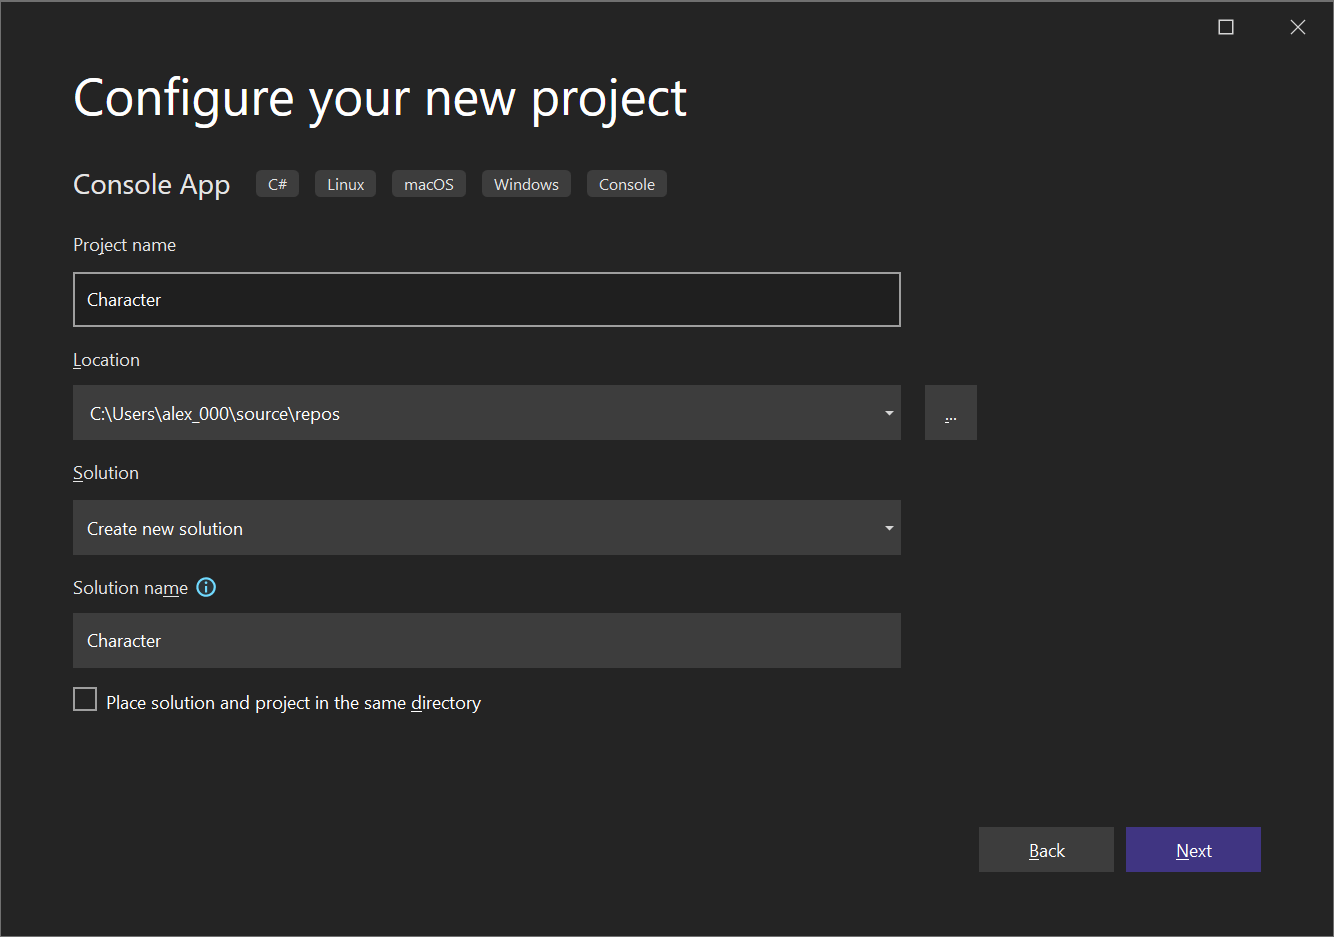
\includegraphics[scale = 0.4]{CharacterClass}

Click "Create". Now, we will create a class for our project. Right-click this in the Solution Explorer window:


\includegraphics{Character}

then click "Add" and then "New Item..."

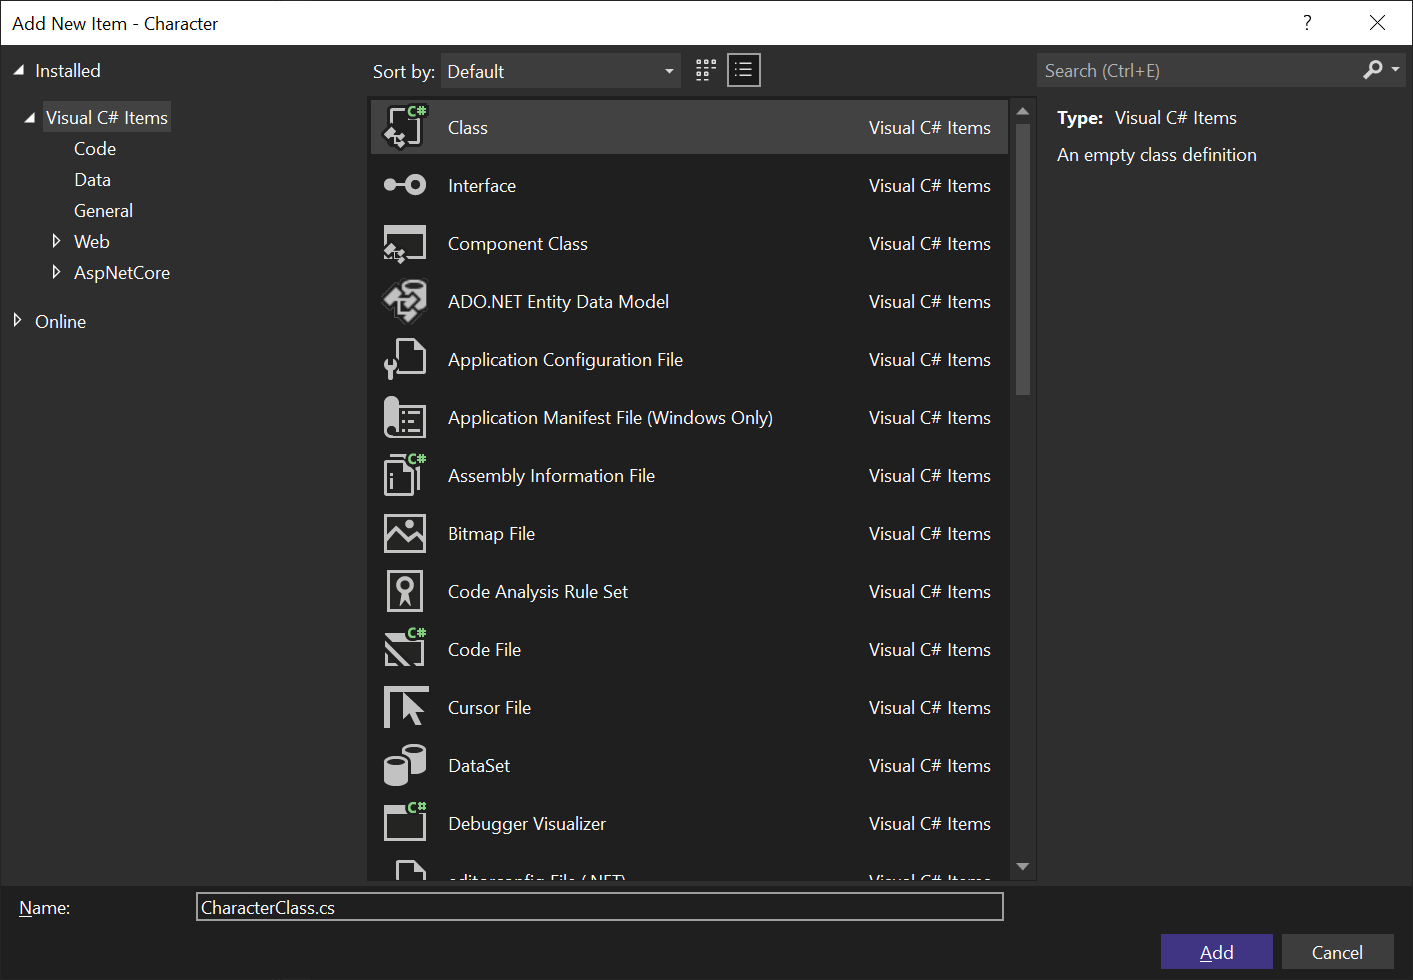
\includegraphics[scale=0.6]{CharacterClassCreator}

Click "Class" and we'll set the name to "Character.cs".

Our code will look like this:
\begin{CSharp}
namespace CharacterClass
{
    internal class Character
    {
    }
}
\end{CSharp}

\section{Creating a Class Constructor}
\index{Class constructor}
Now, let's make our class constructor; this allows us to create Character objects. Let's add this to our Character class:

\begin{CSharp}
public Character()
{}
\end{CSharp}
Hooray! Let's test out what we have so far. 

CLick "Program.cs" in Visual Studio, and create a character object. We can create an object the same way we've created other non-static class objects.

\begin{CSharp}
Character character1 = new Character();
\end{CSharp}

The "new Character();" section calls our class constructor, which creates a Character object. It then sets that to the value of "character1".
However, our class does not have many features by default. Try accessing the methods of "character1" and you'll see a few, such as ToString and GetHashCode. All classes have these methods built-in.

The rest of this chapter will concern adding features to our class.

Let's think of aspects that an RPG character would have. They would likely have various attributes, such as int variables that contain information concerning their strength, intelligence, and other aspects. Let's think about implementing these in our class.

\section{Fields and Properties}
An important aspect of classes that we must know is how variables are stored in them. Properties allow us to access our variable information outside of our class file. When properties are set and retrieved in our program, we access their internal implementation -- these are called "fields".

Here's how we might create a field for a "strength" integer variable:

\begin{CSharp}
private int strength;
\end{CSharp}

The use of the word "private" indicates that the variable can't be accessed within our program itself. We'll use properties to manage how our program can access our variable.

Within properties, there are two aspects that we need to think about: getting the value of our variable and setting it in our program. Here's how our Strength property will look like:

\begin{CSharp}
public int Strength
    {
        get { return strength; }
        set { strength = value; }
    }
\end{CSharp}

Let's work with this in our program by trying to set the Strength in Main:

\begin{CSharp}
character1.Strength = 5;
\end{CSharp}

Since we are setting the value of character1.Strength, the "set" aspect of our Strength property is accessed. We get the value 5 and set our internal strength variable equal to that.

If we were to access the value of character1.Strength like this:

\begin{CSharp}
Console.WriteLine(character1.Strength);
\end{CSharp}

we would be accessing the "get" feature of Strength. In this case, it would return the value of the private variable "strength".

Let's make one quick addition before we expand more on classes; it is considered standard for our private variables to have an underscore at the beginning of the name, which differentiates it more from the public property which is capitalized:

\begin{CSharp}
private int _strength;
\end{CSharp}

\exercise
Create additional fields and properties for our class that correspond to other character attributes.

\exercise
Create an additional constructor that accepts arguments for all the character attributes and sets them within the constructor's curly brackets. In your Main program, try creating a new Character object with that constructor.

\exercise
Extend our program to have more properties. What other elements might a Character have?
\section{Methods}
Earlier, we had a brief chapter concerning methods. The intent was to allow you to understand and use pre-made methods in your code, like Console.WriteLine or Int32.TryParse. Since we're moving into making our own classes, this gives us a better opportunity to utilize methods.

For example, suppose we had a property and field to manage health:
\begin{CSharp}
private int health;

public int Health
{
    get
    {
        return health;
    }
    set
    {
        health = value;
    }
}
\end{CSharp}
and we wanted to be able to decrease the health of another character.

We could write a method like this:
\begin{CSharp}
public int attack(Character opponent, int damage)
{
  opponent.Health -= damage;
}
\end{CSharp}
In the file with our Main method, we could initialize our health and take damage like this:

\begin{CSharp}
Character character1 = new Character();

character1.Health = 100;

Character character2 = new Character();

character2.Health = 50;

character1.attack(character2, 30);
\end{CSharp}
\exercise
What will character2's health be at the end of the above code?
\exercise
Make our attack method only work if the other character is not "defeated". If it is, output a message to that effect in the Attack method.

\section*{Going from Here}
The next chapter will cover exception handling, which is used to handle potential errors that can occur when running your programs.
\chapter{Exception Handling}
\minitoc
\section{Introduction}
\index{Exception handling}
Suppose we are designing a method that, for example, is meant to output, line-by-line, the contents of a file. The method will have a string parameter that corresponds to the name of the file that we want to read from. We might start with something like this:

\begin{CSharp}
void outputFile(string fileName)
{
    using (StreamReader rd = new StreamReader("fileName"));
    {
      Console.WriteLine(rd.ReadLine());
    }
}
\end{CSharp}
We could call it like this:
\begin{CSharp}
Console.WriteLine("Enter in a file name and extension (for example, "text.txt": );
string fileName = Console.ReadLine();

while (!File.Exists(fileName))
{
  Console.WriteLine("Your file name is incorrect. Please try again.");
  
  fileName = Console.ReadLine();
}
outputFile(fileName);
\end{CSharp}
This is good. If we were making a program that focused on obtaining file names from user input, this would work.

\index{Exception handling!with the Character class}
However, what should we do if the file name was \emph{not} obtained from the user? For example, what if we were writing a program to create and save Character information -- where Character is a class we made in the Classes chapter. When the user starts the program, they will be given the opportunity to either create a group of Characters which will be saved in a particular file, or display the contents of the already-saved file. 
Here is what the text file could look like:
\begin{verbatim}
10
30
50
60
70

20
30
40
50
60
\end{verbatim}

where each line corresponds to a particular property for a Character.


\begin{CSharp}
Character[] characterArray; = new Character[100];
string inputFile = "input.txt";
Console.WriteLine("This program obtains information from a file.");

using (StreamReader rd = new StreamReader(inputFile)
{
//EndOfStream indicates end of file
for (int i = 0; !rd.EndOfStream; i++)
    {
      characterArray[i].Strength = Convert.ToInt32(rd.ReadLine());
      
      characterArray[i].Intelligence = Convert.ToInt32(rd.ReadLine());
      
      characterArray[i].Penmanship = Convert.ToInt32(rd.ReadLine());
      
      characterArray[i].Fortitude = Convert.ToInt32(rd.ReadLine());
      
      characterArray[i].Metabolism = Convert.ToInt32(rd.ReadLine());
      
      rd.ReadLine(); //Read in the blank line and do nothing with it
    }
}
\end{CSharp}
We may notice some issues with this code. Here are some:
\begin{itemize}
    \item What if our array is too small?
    \item What if our program could not find inputFile?
    \item What if the file can be found, but it contains content in an invalid format?
    \item What if the file can be found, but it is empty?
\end{itemize}
The first one can be solved by using our array resizing technique outlined in our array chapter.

\begin{CSharp}
 for (int i = 0; !rd.EndOfStream; i++)
    {
    if (characterArray.Length < i)
{
        characterArray = arrayResize(characterArray); //Use our solution from the array 
        //exercise
}
       characterArray[i].Strength = Convert.ToInt32(rd.ReadLine());
       
      characterArray[i].Intelligence = Convert.ToInt32(rd.ReadLine());
      
      characterArray[i].Penmanship = Convert.ToInt32(rd.ReadLine());
      
      characterArray[i].Fortitude = Convert.ToInt32(rd.ReadLine());
      
      characterArray[i].Metabolism = Convert.ToInt32(rd.ReadLine());
      
      rd.ReadLine();
}

\end{CSharp}

Creating this check ensures that our program does not throw an exception for having an array that is too small.

We have our other three issues to deal with. Solving these require more nuance, though, because we are not encountering an issue with our programming: it is with our file. We solved our earlier issue by effectively increasing our array size, but if there is no file, or no data in the text file, we cannot output anything. There is nothing to write to the screen.

\exercise
Try running the program two times, trying to cause the second and third issues. What happens? Bonus: Try to determine what happens with the fourth issue.

Hint: You can create the "input.txt" file in your program's \textbackslash bin\textbackslash debug\textbackslash net(number) directory to test the third example.


Note the exceptions that occur when running your program.

If you completed the above exercise, you might have determined this for the second to fourth issues:
\begin{itemize}
    \item The first results in a System.IO.FileNotFoundException.
    \item The second results in a System.FormatException.
    \item The third skips the loop altogether.
\end{itemize}
Now, let's try to fix these.
\section{An Implementation of Exception Handling}
The FileNotFoundException and FormatExceptions are examples of \emph{exceptions}. They are errors that, by default, force our program to crash when they are thrown.

Luckily, just because how program throws those errors doesn't mean our program has to crash. Now is the time to learn about a C\# feature: try and catch blocks.

First, let's enclose our using section in a try block.
\index{try}
\begin{CSharp}
try{
        for (int i = 0; !rd.EndOfStream; i++)
        {
    if (characterArray.Length < i)
    {
        characterArray = arrayResize(characterArray); //Use our solution from the array 
        //exercise
    }
      characterArray[i].Strength = Convert.ToInt32(rd.ReadLine());
      characterArray[i].Intelligence = Convert.ToInt32(rd.ReadLine());
      characterArray[i].Penmanship = Convert.ToInt32(rd.ReadLine());
      characterArray[i].Fortitude = Convert.ToInt32(rd.ReadLine());
      characterArray[i].Metabolism = Convert.ToInt32(rd.ReadLine());
      
      rd.ReadLine();
    }

}
\end{CSharp}

We enclose our code in try blocks if we think that an exception might be thrown in that particular section of our program.
\index{catch}
Now, we need catch blocks to correspond to each potential exception we anticipate our code throwing.

\begin{CSharp}
try{

    for (int i = 0; !rd.EndOfStream; i++)
        {
    if (characterArray.Length < i)
    {
        characterArray = arrayResize(characterArray); //Use our solution from the array 
        //exercise
    }
      characterArray[i].Strength = Convert.ToInt32(rd.ReadLine());
      characterArray[i].Intelligence = Convert.ToInt32(rd.ReadLine());
      characterArray[i].Penmanship = Convert.ToInt32(rd.ReadLine());
      characterArray[i].Fortitude = Convert.ToInt32(rd.ReadLine());
      characterArray[i].Metabolism = Convert.ToInt32(rd.ReadLine());
      
      rd.ReadLine();
    }
}
catch (System.IO.FileNotFoundException)
{
}
catch (System.FormatException)
{
}
\end{CSharp}

When our program encounters a FileNotFoundException, our program will stop executing the code in our try block and move over to the FileNotFoundException block. Similarly, if our program encounters a FormatException, any code in the FormatException block will run.
\exercise
Try including Console.WriteLine sections in each of our catch blocks, then repeat Exercise 9-1.

\noindent\rule{12cm}{0.4pt}

What might we want to do in the catch blocks? Let's think of why we wanted to catch these issues: because we wanted to handle the case where there were no characters, or the data file was corrupted. If you recall our plans for the program, we decided we wanted to allow users to create characters, or list characters. So, if there was an error that caused no characters to display, why not call the code that allows the player the player to create their own characters.

Supposing that we created a method where users could create and save their own Characters called "createCharacters()":
\begin{CSharp}
catch (System.IO.FileNotFoundException)
{
  createCharacters();
}
catch (System.FormatException)
{
  createCharacters();
}
\end{CSharp}
\exercise
Implement the other main parts of our program. When the user starts the program, ask them if they want to create a list of characters, or list all of the characters in a file.

If they choose the former, call the createCharacters() method. In it, read a group of character properties. When the user enters in a group, ask them if they want to add another character, have our program call a method to list the current characters, or exit the program.

The list code will expand on our sample code. Include it in a method called listCharacters(). After we've saved our lines into our characterArray, display the contents of our array like this:
\begin{verbatim}
Character 1
    Strength: 5
    Intelligence: 3
    Penmanship: 7
    Fortitude: 2
    Metabolism: 3
Character 2
...and so on.
\end{verbatim}
Then, prompt the user to type in a key to exit the program.
\section{Throwing exceptions}
\index{throw}
There is one more possibility that we need to deal with in our list method before we are done. Here it is again:
\begin{itemize}
    \item What if the file \emph{can} be found, but it is empty?
\end{itemize}
Indeed, our program will not throw an exception by default. So, let's manually make our program throw an exception.

Let's go back to our list method. Add this near the top, after we initialize the \emph{inputFile} variable.
\index{FileInfo}
\begin{CSharp}

if (new FileInfo(inputFile).Length == 0)
{
}
\end{CSharp}
We can get the length of the file just by creating a new FileInfo object and giving it our filename. If it \emph{is} empty, its length will be 0: there's no elements.

Now, let's throw an exception. The one that makes the most sense out of our the various types of exceptions we can throw is the NullReferenceException. This indicates that a variable has no value.

\begin{CSharp}
if (new FileInfo(inputFile).Length == 0)
{
  throw new NullReferenceException();
}
\end{CSharp}

Then, we need to catch our exception. So, our exceptions list will now look like this:

\begin{CSharp}
catch (System.IO.FileNotFoundException)
{
  createCharacters();
}
catch (System.FormatException)
{
  createCharacters();
}
catch (System.NullReferenceException)
{
}
\end{CSharp}

We can call createCharacters() in that block.

\section*{Going from Here}
Next chapter will concern collections that make it easier than ever to store collections of data: Lists and Dictionaries.
\chapter{Lists and Dictionaries}
\minitoc
\index{List}
\section{What are lists?}
Lists are very similar to arrays; however they are more versatile. Here's how we can create a List of strings:

\begin{CSharp}
List<string> newList = new List<string>();
\end{CSharp}

One of the main benefits of Lists over arrays is that their sizes can increase as we add elements to them. When arrays are initialized, they are given a predefined length. Here's how we can add a value to our list:
\begin{CSharp}
newList.Add("This is a string");
\end{CSharp}

Suppose we wanted to create a collection for the test scores of a particular student. Since Lists can change sizes, we don't need to think about the maximum number of scores:

\begin{CSharp}
List<double> studentTestScores = new List<double>();
Console.WriteLine("Please enter the student's test grades.");
Console.WriteLine("Follow each number by pressing the "Enter" key.");
Console.WriteLine("Press enter on a line if you are done.");

while (Double.TryParse(Console.ReadLine(), out double grade)
{
  studentTestScores.Add(grade);
}
\end{CSharp}
We could have used an array here. However, we would have had to create an index value that increased by one to keep track of the array element to initialize.
We also don't know how many scores will be inputted. With an array, we could indeed copy our contents into progressively larger arrays as we needed more elements, but this is resource-intensive.

\exercise
Output the values to a text file, as well as the average of all the test scores. We can use the Count property of Lists to get the number of items.

\exercise
Write a program that creates Characters, which we defined in our Class chapter. At the end of each created character add the Character to a list and ask the user if they would like to make another one; if they input an affirmative answer, repeat the character creation code (A do-while loop would be useful here).

\exercise
View the Microsoft documentation on Lists here:

\url{https://docs.microsoft.com/en-us/dotnet/api/system.collections.generic.list-1?view=net-6.0}

With this article in mind, create a program that reads in a string with Console.ReadLine() and puts any values that can be converted to integers into the List. Hint: you can use a foreach loop to access each element of our string:

\begin{CSharp}
foreach (char letter in numberString)
{

}
\end{CSharp}

Then, remove the last integer. For the last step, display the number of elements of the List.

\section{Dictionaries}
\index{Dictionary}
Suppose we wanted to store a collections of multiple, interrelated items. For example, we might want to store a list of products and their corresponding prices. We could set up our data like this:
\begin{CSharp}
List<string> itemNames;
List<double> itemPrices;
\end{CSharp}
We could Add itemNames and itemPrices in the same order in their respective Lists, knowing that if were to use the same index, we could access both properties.

What if there was an easier way to organize this? Instead of keeping two Lists, wouldn't it be easier to store both aspects in one object? Luckily for us, there is: the Dictionary. Dictionaries are similar to Lists, except that elements are indexed not by an integer, but by a more meaningful value.

We can store our item and itemPrices values like this:
\begin{CSharp}
Dictionary<string, double> items = new Dictionary<string, double>();
\end{CSharp}
\index{Dictionary!Add()}
We can add elements similarly to a List; here, we accommodate both of the properties. Here are some examples of adding items:
\begin{CSharp}
items.Add("Water Bottle", 3.50);
items.Add("Toilet Paper", 2);
\end{CSharp}
The first argument that we give to add is referred to as a Dictionary's key, while the second is called the value. That is, we use a "key" to access a particular value.

The power of dictionaries comes with the fact that we can access our values in more meaningful ways than using integers. For example, since we added an element with the key "Water Bottle" with a value of 3.5:
\begin{CSharp}
Console.WriteLine(items["Water Bottle"]);
//The above line outputs "3.5"
\end{CSharp}
If we were using a List, we would have had to use integers to obtain values. It makes more sense that we would use a Dictionary in this scenario, because it is clearer to access our prices through the product names than to use integers, which do not meaningfully relate to their values.

Although Dictionary values can be accessed similarly to Lists and arrays, it is more common to use a Dictionary's TryGetValue method:
\index{Dictionary!TryGetValue()}
\begin{CSharp}
items.TryGetValue("Water Bottle", out double value);
Console.WriteLine(value);
\end{CSharp}

TryGetValue is preferred because this method returns a Boolean indicating a given value was found in the Dictionary:

\begin{CSharp}
Console.WriteLine("Enter in a product name. This program will return the price.");
int result;
while (!items.TryGetValue(Console.ReadLine(), out result)
{
  Console.WriteLine("The product you entered in is invalid. Please try again.");
}
Console.WriteLine(\$"The price is \${result}");
\end{CSharp}

We can also remove items from our list using the Remove method:
\index{Dictionary!Remove()}
\begin{CSharp}
items.Remove("Water Bottle");
\end{CSharp}
Given the Dictionary defined in our previous examples, this removes the key "Water Bottle" and its associated value: 3.50.

\exercise
Implement the full shopping list program using a Dictionary.

\noindent\rule{12cm}{0.4pt}
During this chapter, we hope you learned the power and features Lists and Dictionaries can give you. Although the concept of arrays are common across multiple programming languages and thus useful to learn, Lists are ultimately more powerful in C\#. Therefore, we will use them more often in future chapters of this book.
\section*{Going from Here}
The next chapter will concern LINQ: a technology that makes it easy to sort and filter through collections of data.

\chapter{LINQ}
\minitoc
\section{Introduction}
Suppose we had a had a list of strings, that we, say, obtain from a file:
\begin{CSharp}
List<string> bookTitles = new List<string>();

using (StreamReader strm = new StreamReader("books.txt"))
{
 bookTitles.Add(strm.ReadLine());
}
\end{CSharp}

and we want to create a new list that consists of all of the strings, but sorted according to their length.

One way we could solve this starts with the knowledge that we can compare strings, like so:
\begin{CSharp}
if (words[0].Length < words[1].Length)
{
  Console.WriteLine(\$Length-wise, {words[0]} occurs before {words[1]}.");
}
\end{CSharp}
and extrapolating this toward the research of any one of the lengthy algorithms to sort an array.

However, what if there was an easier way that took advantage of C\#'s features? Luckily for us, there is.
\index{LINQ}
LINQ, or Language Integrated Query, gives us a powerful toolset for sorting, grouping, and doing other organizational tasks. In practice, LINQ gives us several methods for us to complete such tasks.

Here is how we could sort our aforementioned list of strings alphabetically, keeping in mind to put "using System.Linq;" at the top of our file.
\index{OrderBy}
\index{IEnumerable}
\begin{CSharp}
IEnumerable<string> sort = bookTitles.OrderBy(book => book.Length);
\end{CSharp}
The OrderBy argument may be a little confusing. What we are indicating is that for each book in bookTitles, we'll call it "book", and organize it according to our book's Length property. The particular word "book" doesn't actually matter: it is just a way I chose to reference an individual element.

Our sort variable does not actually contain the re-ordered book titles. It just saves the contents of the query that we want on the bookTitles list.

To actually execute our OrderBy query, we need to use the ToList method on our IEnumerable variable.
\index{ToList}
\begin{CSharp}
List<string> sortedList = sort.ToList();
\end{CSharp}

It might seem unintuitive that the actual query is stored separately from our sorted list. However, this separation between our query and our values allow us to run our query again after editing our list:

\begin{CSharp}
IEnumerable<string> sort = bookTitles.OrderBy(book => book.Length);

List<string> sortedList = sort.ToList();

bookTitles.Add("War and Peace");

List<string> sortedList2 = sort.ToList();
\end{CSharp}


Note that we didn't change anything in the query since we first defined it. The only thing that sort knows is that it needs to "look at the bookTitles List and sort it"; the query details are independent of what's in our actual List. When we first run "sort" it does what we defined it to do, and it is doing the same when we run it again. So, since we added an element to bookTitles after we ran it the first time, the second time we execute our query we'll obtain a result containing our new element.

If we want to execute our query without storing the result, we can simply use a foreach loop on our IEnumerable object:
\begin{CSharp}
foreach (string sortedBook in sort)
{
    Console.WriteLine(sortedBook);
}
\end{CSharp}
\section{Where}
\index{Where}
There are many more methods than OrderBy. Suppose we wanted to obtain a subset of elements from our List<string> that had a particular search term, and add them to a new List. If we look at the C\# documentation for strings, we can see that the Contains method returns a Boolean if a string contains a particular given string. If we decided not to use LINQ, we might write this:

\begin{CSharp}
//Suppose "list" is defined earlier on

string wordToFilter = Console.ReadLine();
List<string> filteredList = new List<string>();

foreach (string word in list)
{
  if (word.Contains(wordToFilter)
  {
    filteredList.Add(word);
  }
}
\end{CSharp}

With LINQ, we can write this much more easily:
\begin{CSharp}
string wordToFilter = Console.ReadLine();
IEnumerable<string> filterByString = list.Where(word => word.Contains(wordToFilter));

List<string> filteredList = filterByString.ToList();
\end{CSharp}


\exercise
Make a program that reads a text file, and asks a user to input a search term. Display the lines that meet the search criteria.
\exercise
Update the previous program so that after the user inputs in their search term, prompts them whether they want lines to be displayed that contain their search term, or if they want the lines that do \emph{not} contain their search term. After they choose an option, display the requisite lines.
\exercise
Expand on your queries from the previous exercise by requiring that the results are ordered. Hint: LINQ queries can be performed on IEnumerable values.

\section{Any}
\index{Any}
The "any" method can be used in two different ways. It can check whether elements exist in a list or other collection, or if any given elements satisfies a condition.

For example, for the former:

\begin{CSharp}
bool areThereElements = bookTitles.Any();
\end{CSharp}

Here's an example of how we might check if any of the elements contain a particular string:

\begin{CSharp}
string wordToFilter = Console.ReadLine();
bool filterByString = list.Any(word => word.Contains(wordToFilter));
\end{CSharp}
Note that the above code is similar to our Where example. However, instead of using a query to retrieve elements with a particular condition, we simply check if such elements exist. It also returns a bool concerning whether they exist or not instead of an IEnumerable for our query.
\section{Group}
Suppose we wanted to create a collection that consists of similar items from a list grouped together. For example, we might want to create a filtered version of a list where elements that meet a specific search term are grouped together.

Here is how we could make such a list:

\begin{CSharp}
List<string> items = new List<string>();
items.Add("Cats");
items.Add("Dogs");
items.Add("Fish");
items.Add("Catfish");
List<IGrouping<bool,string>> filter =
items.GroupBy(word => word.Contains("Cat")).ToList();

Console.WriteLine(filter);
\end{CSharp}
The filter variable is a bit complicated. To use the GroupBy method, the types of elements in our list need to be IGrouping elements. Since we want to filter our list based on whether or not our values meet a criteria and our list is made up of strings, we use IGrouping<bool, string>.

We can use the debugger (see chapter 5) to easily see what our list looks like. Create a statement after the creation of the list so we can put a breakpoint there -- for example, a Console.WriteLine(). After you place the breakpoint, run the program and look at the watch panel:

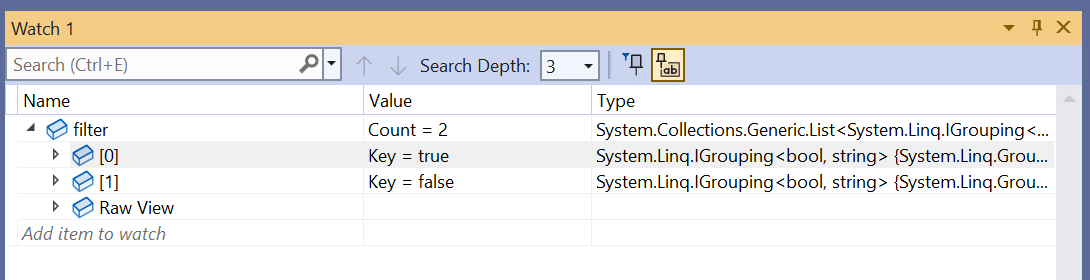
\includegraphics[scale=0.33]{groupbydebugger1}

You can see that our list has two elements: a true and a false value. If we expand with the arrow icons on the left, we can further see that each element consists of elements of our original list, organized according to whether they meet the condition of containing the word we used.
\section*{Continuing from Here}
For the next chapter we'll delve into graphical programs, which is at the forefront of modern consumer applications.
\chapter{Introduction to Graphical Programs}
\minitoc
\index{WPF}
In previous chapters, we have covered writing programs in the context of console applications, which allowed us to purely focus on the logic of our programs without needing to concern ourselves with a user interface.

As you likely know, most applications we use today use a graphical user interface, which allow us to navigate programs with the use of our mouse. Instead of typing information into a text console, we can click, scroll, and do all of the actions expected in modern applications.

Let's start now.
\section{Setting up our Graphical Application}
When starting Visual Studio, create a new project and choose "WPF Application". Then, click "Next" and name it "My First GUI Application."

When you continue past these menus, you should see a screen that looks like this:


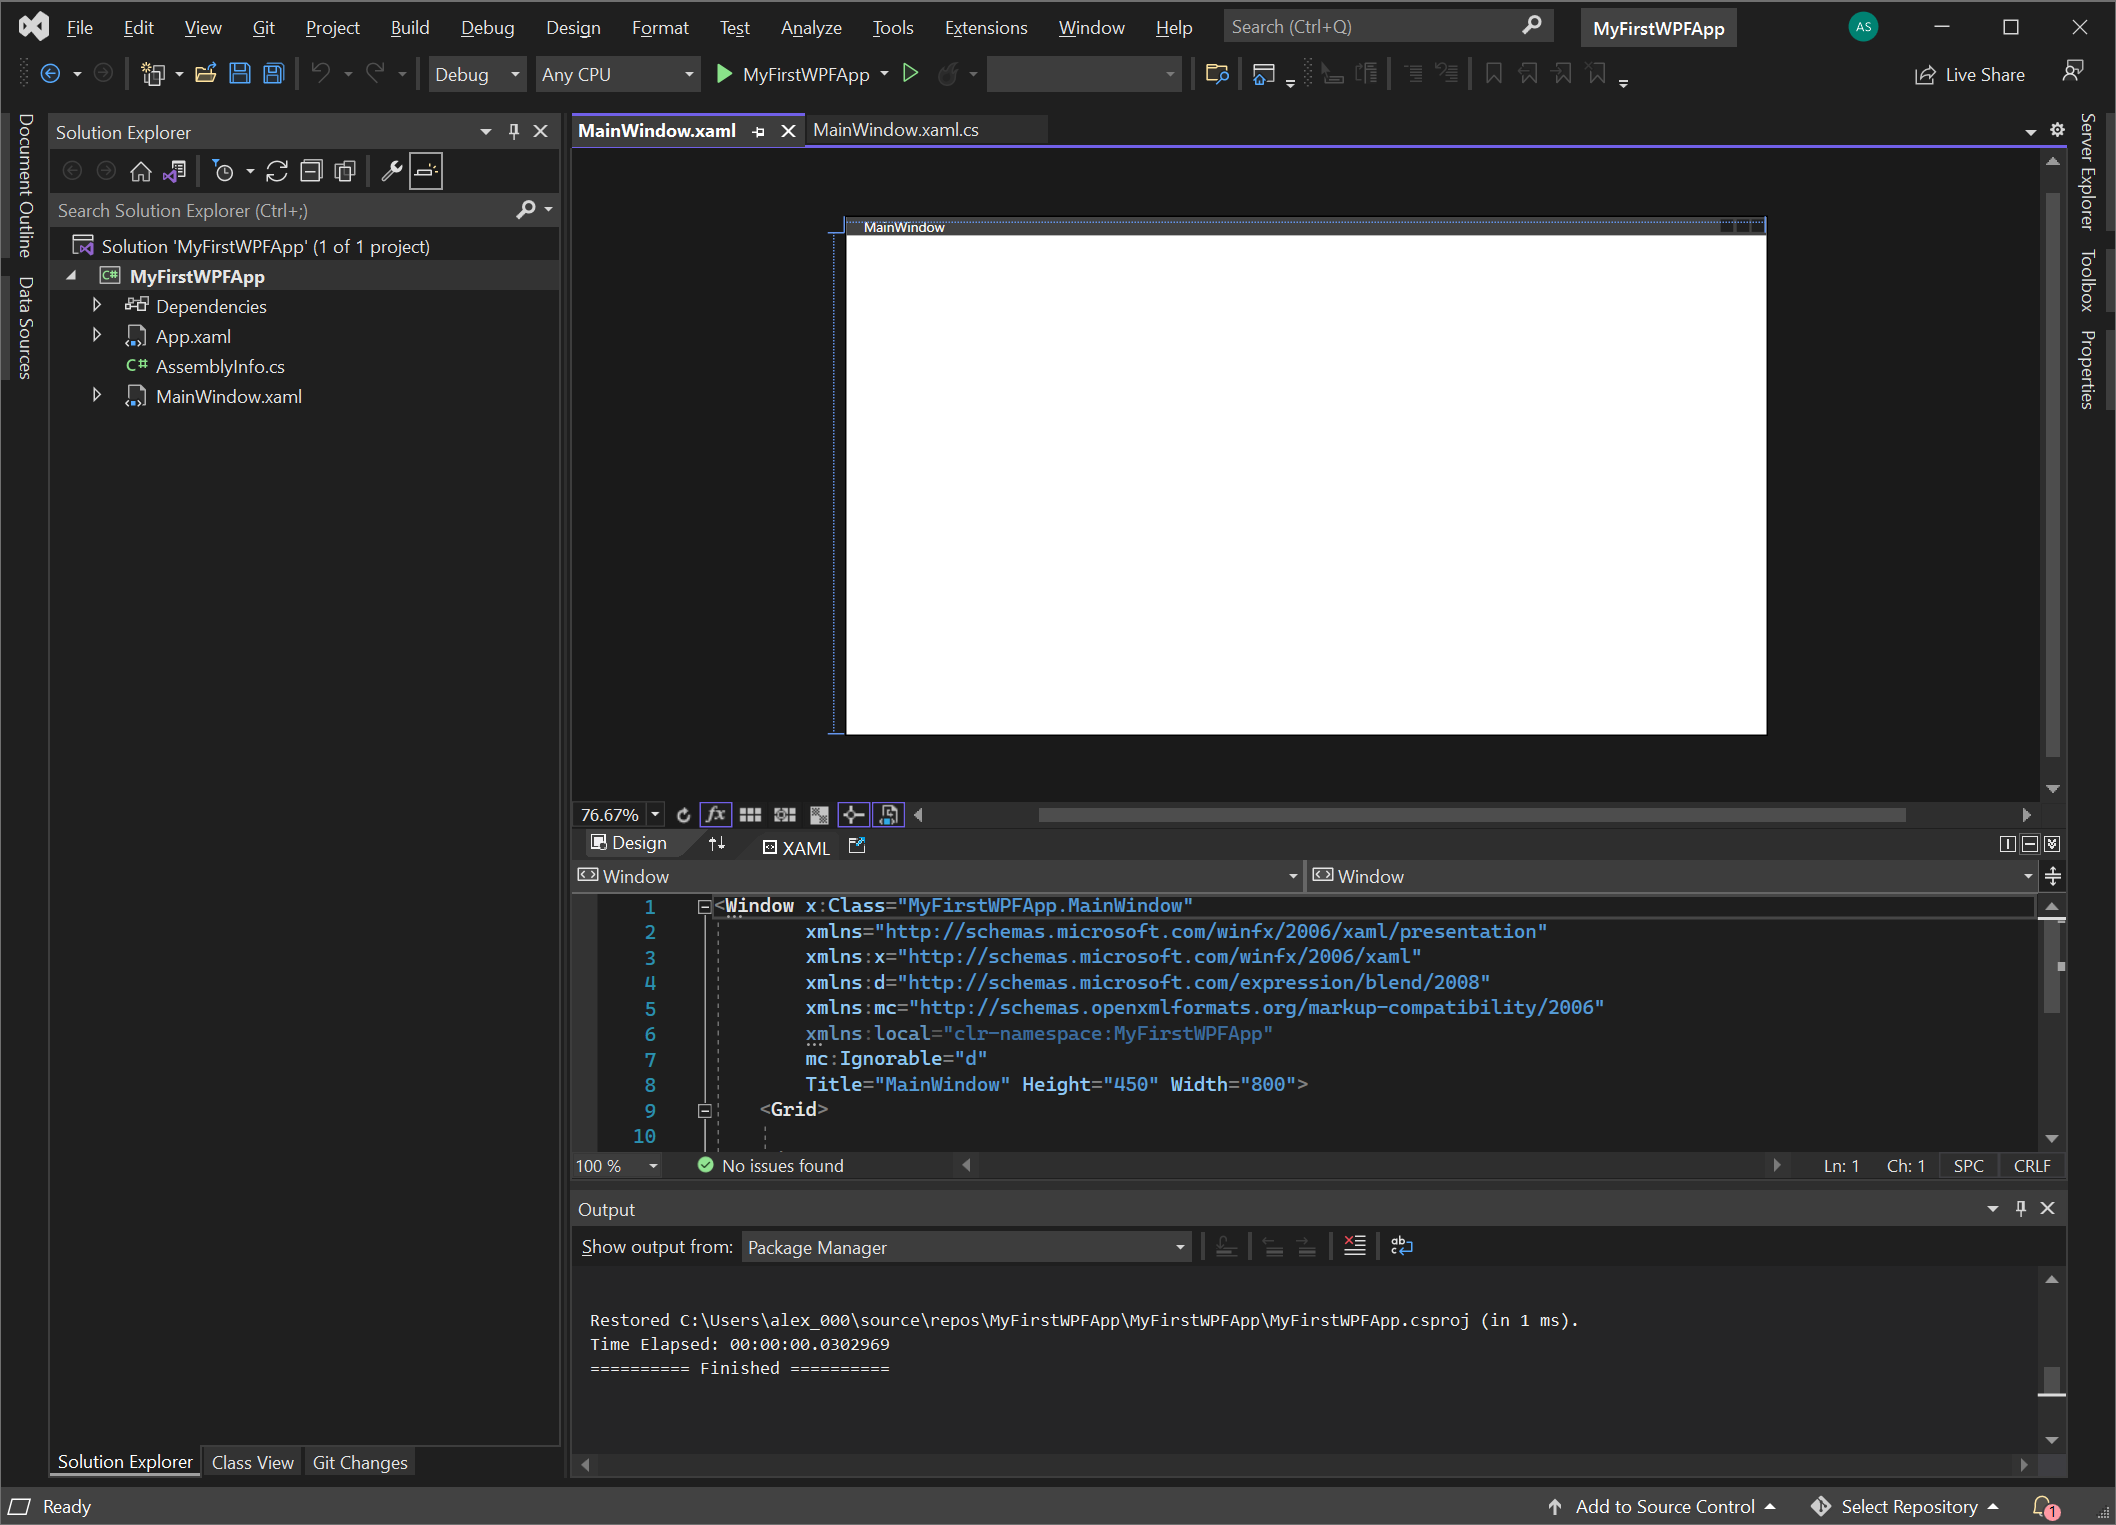
\includegraphics[scale = 0.2]{WPF}

Hooray, we have the base of our GUI application up. Let's continue by adding a button. They are a fundamental feature of GUI applications.

First, go to the left-hand side of the screen and click "Toolbox". Click "Button". Click the triangle to the left of "All WPF Controls" if it's not enabled, and choose "Button" out of the list.

Note that we didn't have to write our button's boilerplate code. Instead, Visual Studio handles this -- we only have to focus on what the button \emph{does} when it is clicked as well as other high-level tasks -- not programming the basics of the button itself.


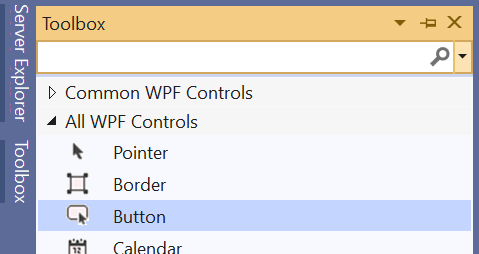
\includegraphics[scale = 1]{FindingButton}

Then, we can simply drag it to our form:

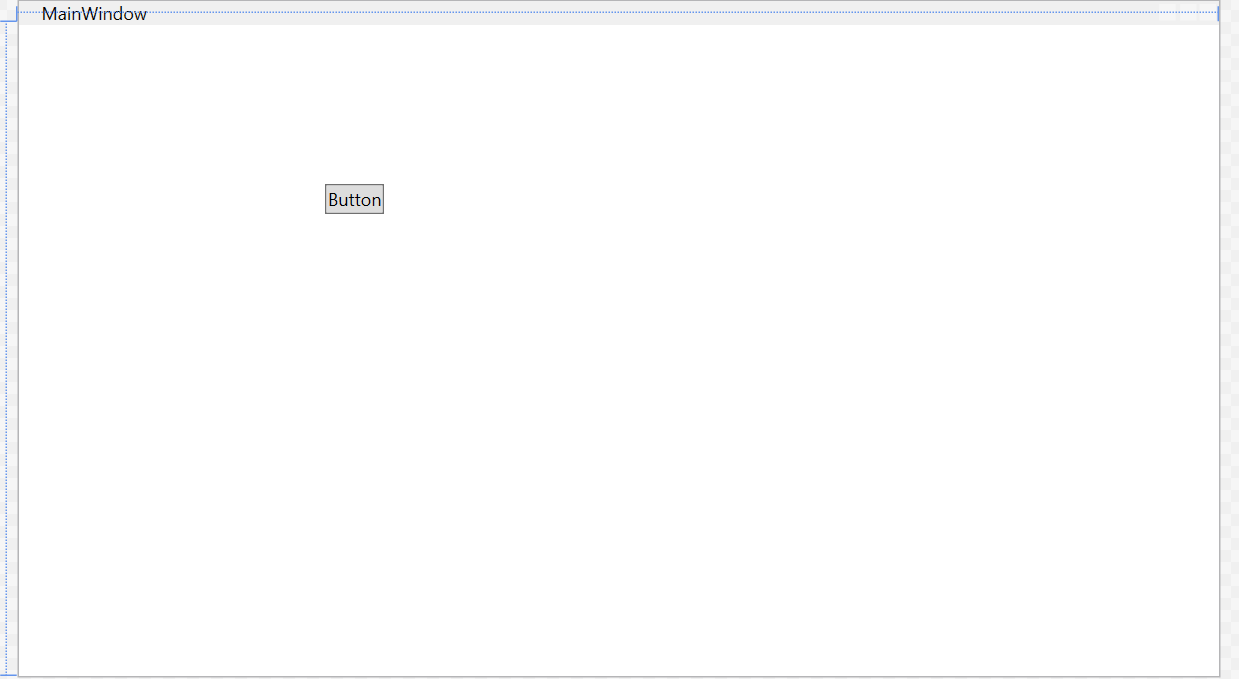
\includegraphics[scale = 0.5]{FormWithButton}

(If your button is too small, you can click the button and drag on the squares that appear to resize it.)
\section{Adding a Button}
\index{Button}
Now, let's get back to C\# programming! We can double-click the button which brings us to a coding window where we can type in what happens when the button is clicked. These blocks of code are called \emph{events}: an action is performed after a user interacts with our application in a particular way.

When we double-click the button, we'll see this:
\begin{CSharp}
private void button_Click(object sender, RoutedEventArgs e)
        {

        }
\end{CSharp}

Let's program a simple application which shows us a message when we click the button. How can we display the message? There is a static class called "MessageBox" that we can use to show our message. We'll use the "Show" method of "MessageBox", which takes a string argument for the message.

\exercise
Use the MessageBox.Show method to show a message of your choice. You can then run the program by clicking the green arrow at the top of Visual Studio (as with our console applications). Try clicking the button.

\par\noindent\rule{\textwidth}{0.4pt}

When running our program, you may see "error CS1061" in the output window at the bottom of the screen. If that occurs, double-click the error and make sure that 
the information between the quotes in

Click=""

matches the name of our event: by default it should contain "button\_click".

Let's make one more update before we go on to some more exercises: we'll change our button's text.

Above our window, click the "MainWindow.xaml" tab to edit our UI. If that tab's not there, go to the Solution Explorer window and double-click "MainWindow.xaml".

Click our button, and you'll see a "Properties" window appear. Use the search bar to search for "Content". This handles the text inside our button. Let's change it to say something like, "Click me for a message."

For these next exercises, feel free to either delete our button and create new ones or make a new program entirely.
\exercise
Create a button that, when clicked, will create a file and write some text (of your choice) with a StreamWriter. After that, display a confirmation that the file was written.

\exercise
Update our application from Exercise 10-2 so that our program will ask the user whether a file should be created before it does it. How can you handle "yes" or "no" buttons for our MessageBox? 
Look at \url{https://docs.microsoft.com/en-us/dotnet/api/system.windows.messagebox?view=windowsdesktop-6.0} for a MessageBox.Show method that will allow us to display those buttons within our MessageBox.
\section*{Going from Here}
In the next section, we will expand over this content by learning about other WPF controls besides buttons and MessageBoxes.

\chapter{XAML and More Controls}
\minitoc
Let's learn about some other graphical elements (typically referred to as "controls") that we can implement with C\# and WPF.

\section{Introduction to XAML}
\index{XAML}
In the previous chapter, we discussed the use of Buttons, where a programmer can drag in items from the Visual Studio Toolbox into their program. However, there is a preferred way of working with UI elements that is faster than using the Toolbox: writing in XAML.

XAML, which stands for "Extensible Application Markup Language", allows us to insert and specify properties of UI elements simply by typing what elements we want displayed and their properties and associated methods.

During the previous chapter, you might have noticed a section of your Visual Studio window that looks like this:


\includegraphics[scale=0.11]{XAMLIntro.png}
\index{<Window>}
This defines the structure of a WPF window. Let's start by trying to add an element: how about a Button?

All of the information regarding our window is enclosed between the lines <window and </Window>. So, to add an element, we need to put our content in between those two portions, or tags. Inside our <Window> elements, we must further place all of our elements between <Grid> and </Grid>; Grid handles alignment for our elements..

So, our XAML will look something like this:

\index{<Grid>}
\begin{verbatim}
    <Window
        xmlns="http://schemas.microsoft.com/winfx/2006/xaml/presentation"
        xmlns:x="http://schemas.microsoft.com/winfx/2006/xaml"
        //and so on...
    <Grid>
    
    </Grid>
</Window>
\end{verbatim}
\index{<Button>}
To add a Button element to our window, add a tag between the two Grid tags that looks like this:

<Button></Button>.

Notice the structure of that tag. Similarly to Window and Grid, the tags are structured by first placing a left angle bracket, followed by a specific type, and then a />.

\index{<Button></Button>!Width}
\index{<Button></Button>!Height}
After you type that, you should see the window change to show our new button. This button can be resized by modifying its height and width attributes. For example, we could change the Width and Height for the button like this:
\begin{verbatim}
<Button Height ="49" Width="114"/>
\end{verbatim}
Note that attributes do not have to be in that particular order. We could have just as easily written
\begin{verbatim}
    <Button Width="114" Height ="49"/>
\end{verbatim}

I recommend using the first choice, since the use of alphabetical order makes it easier to read.
\exercise
Try modifying our button to extend across the screen horizontally. Then, undo that (press ctrl+z), and make it so it extends across the screen vertically. After you're done, reset it back to normal.
\par\noindent\rule{\textwidth}{0.4pt}
We can also move the button around with the Margin property, which describes the amount of space between the window and an element. We can set four values: right, up, left, and down.
\begin{verbatim}
    <Button Width="114" Height ="49", Margin="200,312,0,0"/>
\end{verbatim}
Imagine there are four rectangles that start at the four corners of our window and extend to our Button, and our Button's default spot is at the top-left (which would represent margin values of 0,0,0,0). If we were to extend our leftmost rectangle to 200 units, it would push our Button away from the top-left corner over to the right. The second would extend the topmost rectangle downward 312 units, which would push our element down. We set the right and bottom to 0 units, so our button's final position is at the bottom-left.

On another note, you might have noticed that the text of our button is listed as "Button". To change the text, edit the Content property.
\index{<TextBox>}
\index{<Label>}
\section{Textboxes and Labels}
Textboxes are very common in graphical applications; they allow users to input text into a program.

We can add a TextBox like this:
\begin{verbatim}
    <TextBox></TextBox>
\end{verbatim}
\exercise
Add a TextBox to your program and try adding text to it.
Then, exit and set the TextBox's Width and Height to more typical values; I recommend values of 51 and 18, respectively.
\par\noindent\rule{\textwidth}{0.4pt}
Another element that you can add is a Label. Unlike Buttons and TextBoxes, what labels do might not be intuitive at first glance. They actually allow you to directly add text into your program: for example, a descriptor describing another element. We can add them similarly to how we did for Buttons and TextBoxes. Like Buttons, we can set their text with the Content property.
\section{A Shopping List Program}
If you recall from earlier chapters, there was a series of exercises that involved managing a shopping list. A user could run a console program that allowed them to input elements, which could be displayed on the screen and edited. How might we write this to work with WPF?

We could display information via Labels, prompting the user to enter in a product. The user could enter in the product and quantity using TextBoxes, and click a Button to submit their item. How could we list these objects? If we do some research through Microsoft's documentation, we might find information concerning ListViews, which gives us a way to display items. This sounds like a useful element for our needs.

Let's add the elements to our program: two TextBoxes, a ListView, and three Labels (one of them is for describing what's in the ListView.
After adding the elements and adjusting their margins, our program might end up looking something like this:


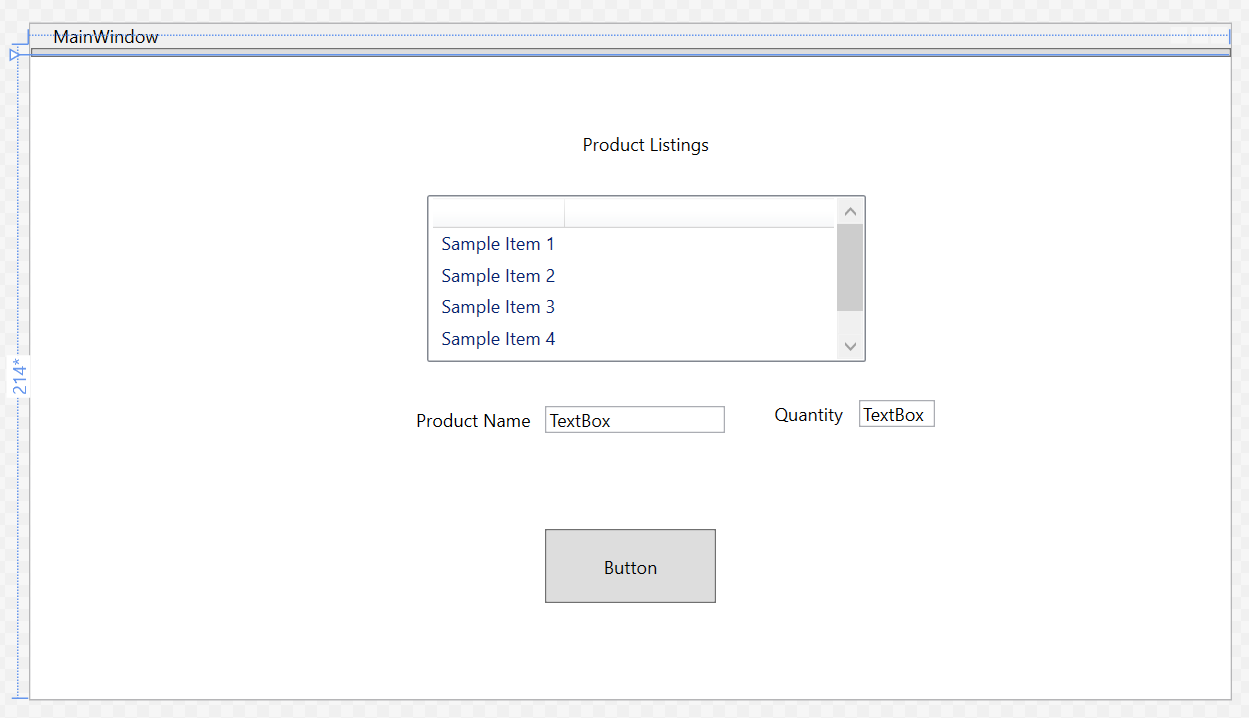
\includegraphics[scale=0.3]{shoppingwpfintro.png}



We need to make some additions to our ListView. By default, ListView simply lists items, but we need to have separate columns: one for the product name, and another for the quantity.

To add columns, we need to first specify that we actually want to edit the View of the ListView -- that is, how the ListView displays elements.

We can do this by entering <ListView.View> between our ListView elements. So, we have:

\begin{verbatim}
  <ListView>
            <ListView.View>
            </ListView.View>
    </ListView>
\end{verbatim}

Then, we need to specify how we want our content to be displayed. As before mentioned, we want our data organized in columns, so we need to use <GridView>:

\begin{verbatim}
    <ListView>
            <ListView.View>
                <GridView>
                </GridView>
            </ListView.View>
    </ListView>
\end{verbatim}
We are close to finishing up our ListView structure; our last step is to specify the data we want in our grid. We know we want two columns: one for the name of the product, and another for the quantity. We can use the GridViewColumn element for this, so between the <GridView> element we'll have:

\begin{verbatim}
    <GridViewColumn Header="Product Name" DisplayMemberBinding="{Binding Name}"/>
    <GridViewColumn Header="Quantity" DisplayMemberBinding="{Binding Quantity}"/>
             
\end{verbatim}
This code means, "When a programmer tries to add an element to this list, get the properties of the element they are trying to add that are named `Name' and `Quantity', and bind them to their respective columns that have the headers `Product Name' and `Quantity.'"

Now, we need to create such a structure that programmers can add to the list with those two properties. It makes the most sense to create a Class that uses a string for our product name, and an integers for our quantity. 

We make our class the same way as we did in Chapter 8, by right-clicking our project in the Solution Explorer, hovering over "Add..." and clicking "New Item", then clicking Class and entering in our class name.

I named my class "Product", and gave it string and integer properties named "Name" and "Quantity", respectively, since they need to match with the DisplayMemberBinding names in the GridViewColumns in order for the values to be detected and added.

Now, we need to do the last few steps, which involves actually taking the content in our TextBoxes and adding them to the list.

Go back to our MainWindow.xaml file and look over at our Button element. We want to program it so that when it is clicked, a C\# method is run that actually adds the elements. We can add a Click attribute for our button to accomplish this. Give it a suitable method name, such as AddElements. Furthermore, go to your TextBoxes and your ListView and add a Name attribute; we need one so we can refer to these variables in our code.

Look over at your Solution Explorer, and click the triangle next to the MainWindow.xaml file. You should see a MainWindow.xaml.cs file appear. This is where we will write our code.

In this file, create a method with the name that you defined in Click. For me, the code is: 
\begin{CSharp}
private void AddProduct(object sender, RoutedEventArgs e)
        {

        }
\end{CSharp}
Do not worry now about what the parameters mean, just know that they need to be added to associate the XAML with our C\#.

We can access the text in our TextBoxes by using their name. For example, if we gave our first TextBox the name "productNameTextBox", we can access it like this,

\begin{CSharp}
private void AddProduct(object sender, RoutedEventArgs e)
        {
            string text = productNameTextBox.Name;
        }
\end{CSharp}

The rest of the program is given in the following exercises:
\exercise
Finish up the addition code for our program. Here is a general guide:
\begin{itemize}
\item The ListView wants an variable with property names of "Name" and "Quantity", so create an instance of our previously-named class and set its values to the two textbox values.

\item We can add an item to a ListView by using its Items.Add method.

\item Remember to check if the value in the quantity TextBox can be converted to an integer before trying to set it for our product. If it cannot, show a MessageBox (as detailed in Chapter 10) with an error message.
\end{itemize}
\exercise
Create deletion functionality, where a user can first click an item and then click a button to delete the selected element. You can get the index of the currently selected item via a ListView's SelectedIndex property, and you can remove an item using a ListView's Items.RemoveAt method, where RemoveAt takes an integer for an index.
\exercise
Create a Save button so the user can save their information to a file.
\section{Radio Buttons and Check Boxes}
\index{<RadioButton>}
\index{<CheckBox>}
Here is what a RadioButton looks like, with text off to the side:
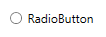
\includegraphics{radiobutton}

Here is what a checkbox looks like:



\includegraphics{checkbox}


If you have experience with Windows or many other operating systems, you might have an intuitive idea of what they do: the former allows you to choose one option out of a set of options, while the latter allows you to choose multiple, or leave the boxes unchecked.

You can create RadioButtons and Check Boxes with the <RadioButton> and <Checkbox> element.

\index{<StackPanel>}
We oftentimes place several of these in an element such as a StackPanel. Adding them in one of these makes it easy to distinguish such elements as part of a group, since each successive element placed in a StackPanel is inserted below the other. Therefore, we do not need to worry about positioning each element ourselves. It also makes it easier to move multiple elements to a different part of the window, since we can just change the margins of its StackPanel.

Here is what a StackPanel with two CheckBoxes might look like:
\begin{verbatim}
    <StackPanel Margin="552,294,0,0">
            <CheckBox Content="CheckBox"/>
            <CheckBox Content="CheckBox"/>
        </StackPanel>
\end{verbatim}
How can our program know when a particular radio button is selected in a series of them? How can we prevent our program from assuming that our radio buttons are separate, and therefore from allowing us to choose several options?

The answer is to use the GroupName attribute. For example:

\begin{verbatim}
    <GroupBox GroupName="First" Content="GroupBox"/>
    
     <GroupBox GroupName="Second" Content="GroupBox"/>
    
        
\end{verbatim}
You can trigger an event for if a CheckBox or RadioButton has been clicked through their "Click" attribute.

Here is how you could examine all of the RadioButtons in a StackPanel, given the StackPanel's name is "panel".

\begin{CSharp}
foreach (UIElement element in panel.Children)
{
  RadioButton button = element as RadioButton;
}
\end{CSharp}
panel.Children retrieves the elements as UIElements, not as RadioButtons. So, since we actually \emph{do} have RadioButton, we need to specifically convert our elements as such so we can examine a button's properties. Our compiler -- the program that is building our program -- does not know are using RadioButtons until we specifically indicate we are with the as keyword.

Why didn't we use TryParse to convert our radio buttons? Why did we use the never-before-seen keyword "as"? Actually, while using a TryParse would be preferable, such a method does not exist for RadioButtons. There is only a TryParse method for a relatively small number of types, like Int and Double.
\exercise
Create a program with several RadioButtons enclosed in a StackPanel. When a radio button is clicked, display a custom message based on the particular button. You can use the Name property to identify specific RadioButtons.
\chapter{Introduction to Relational Databases}
\minitoc
\index{Database}
\index{Database!Relational}
In previous chapters, we have considered the concept of storing data in terms of text files. Such files actually constitute a \emph{database}; an electronic, organized collection of data.
With this in mind, lets consider a more complex form of database: the \emph{relational database}.

Imagine that you wanted to store, for example, a list of employees for a company. You want to include their name and their home address. You also want to have information relating to their job: their title and a job description. Our first idea for an implementation might be to save a file that has those contents: for example,

\begin{verbatim}
    Name: John Smith
    Address: 5555 Computer Dr.
    Job Title: Frontend Web Developer
    Job Description: This job concerns developing the client-side
    part of our website using HTML, CSS, and JavaScript.
    
    Name: James Smith
    Address: 4444 Computer Pkwy.
    Job Title: Backend Web Developer
    Job Description: This job concerns developing the server-side 
    part of our website using PHP and SQL.
    
\end{verbatim}
This code can get messier if we add more employees; as more people acquire a job with the same title, we have to store separate instances of their job description for each person. Furthermore: what happens if one of our job duties change? We will have to change the job description field for every person who is in that position. It's also not immediately obvious how we would handle other fields relating to the job, such as the minimum and maximum pay. This is a file to store employee information: not general job details.

It allows us to create multiple files, and specify how these files might be linked to each other. For example, we might have one file to handle employee information, where we'll focus on the elements specifically related to the employee, while another file relates to job details.

\section{Setting up a Relational Database}

Let's first create a WPF project. Start up Visual Studio, and choose to make a WPF Application as usual. I named my program "Employee Program."

After you create your project, we need to install a package. This package will give us classes and methods that allow us to create and initialize a relational database. Look over at the Solution Explorer tab:

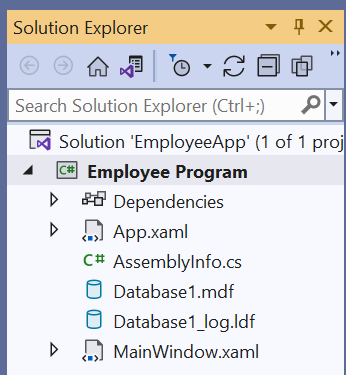
\includegraphics[scale=0.5]{EmployeeProgram}
\index{NuGeT}

Right-click the Dependencies section, and choose "Manage NuGet Packages..."
You'll see this window:

\index{SQLite}
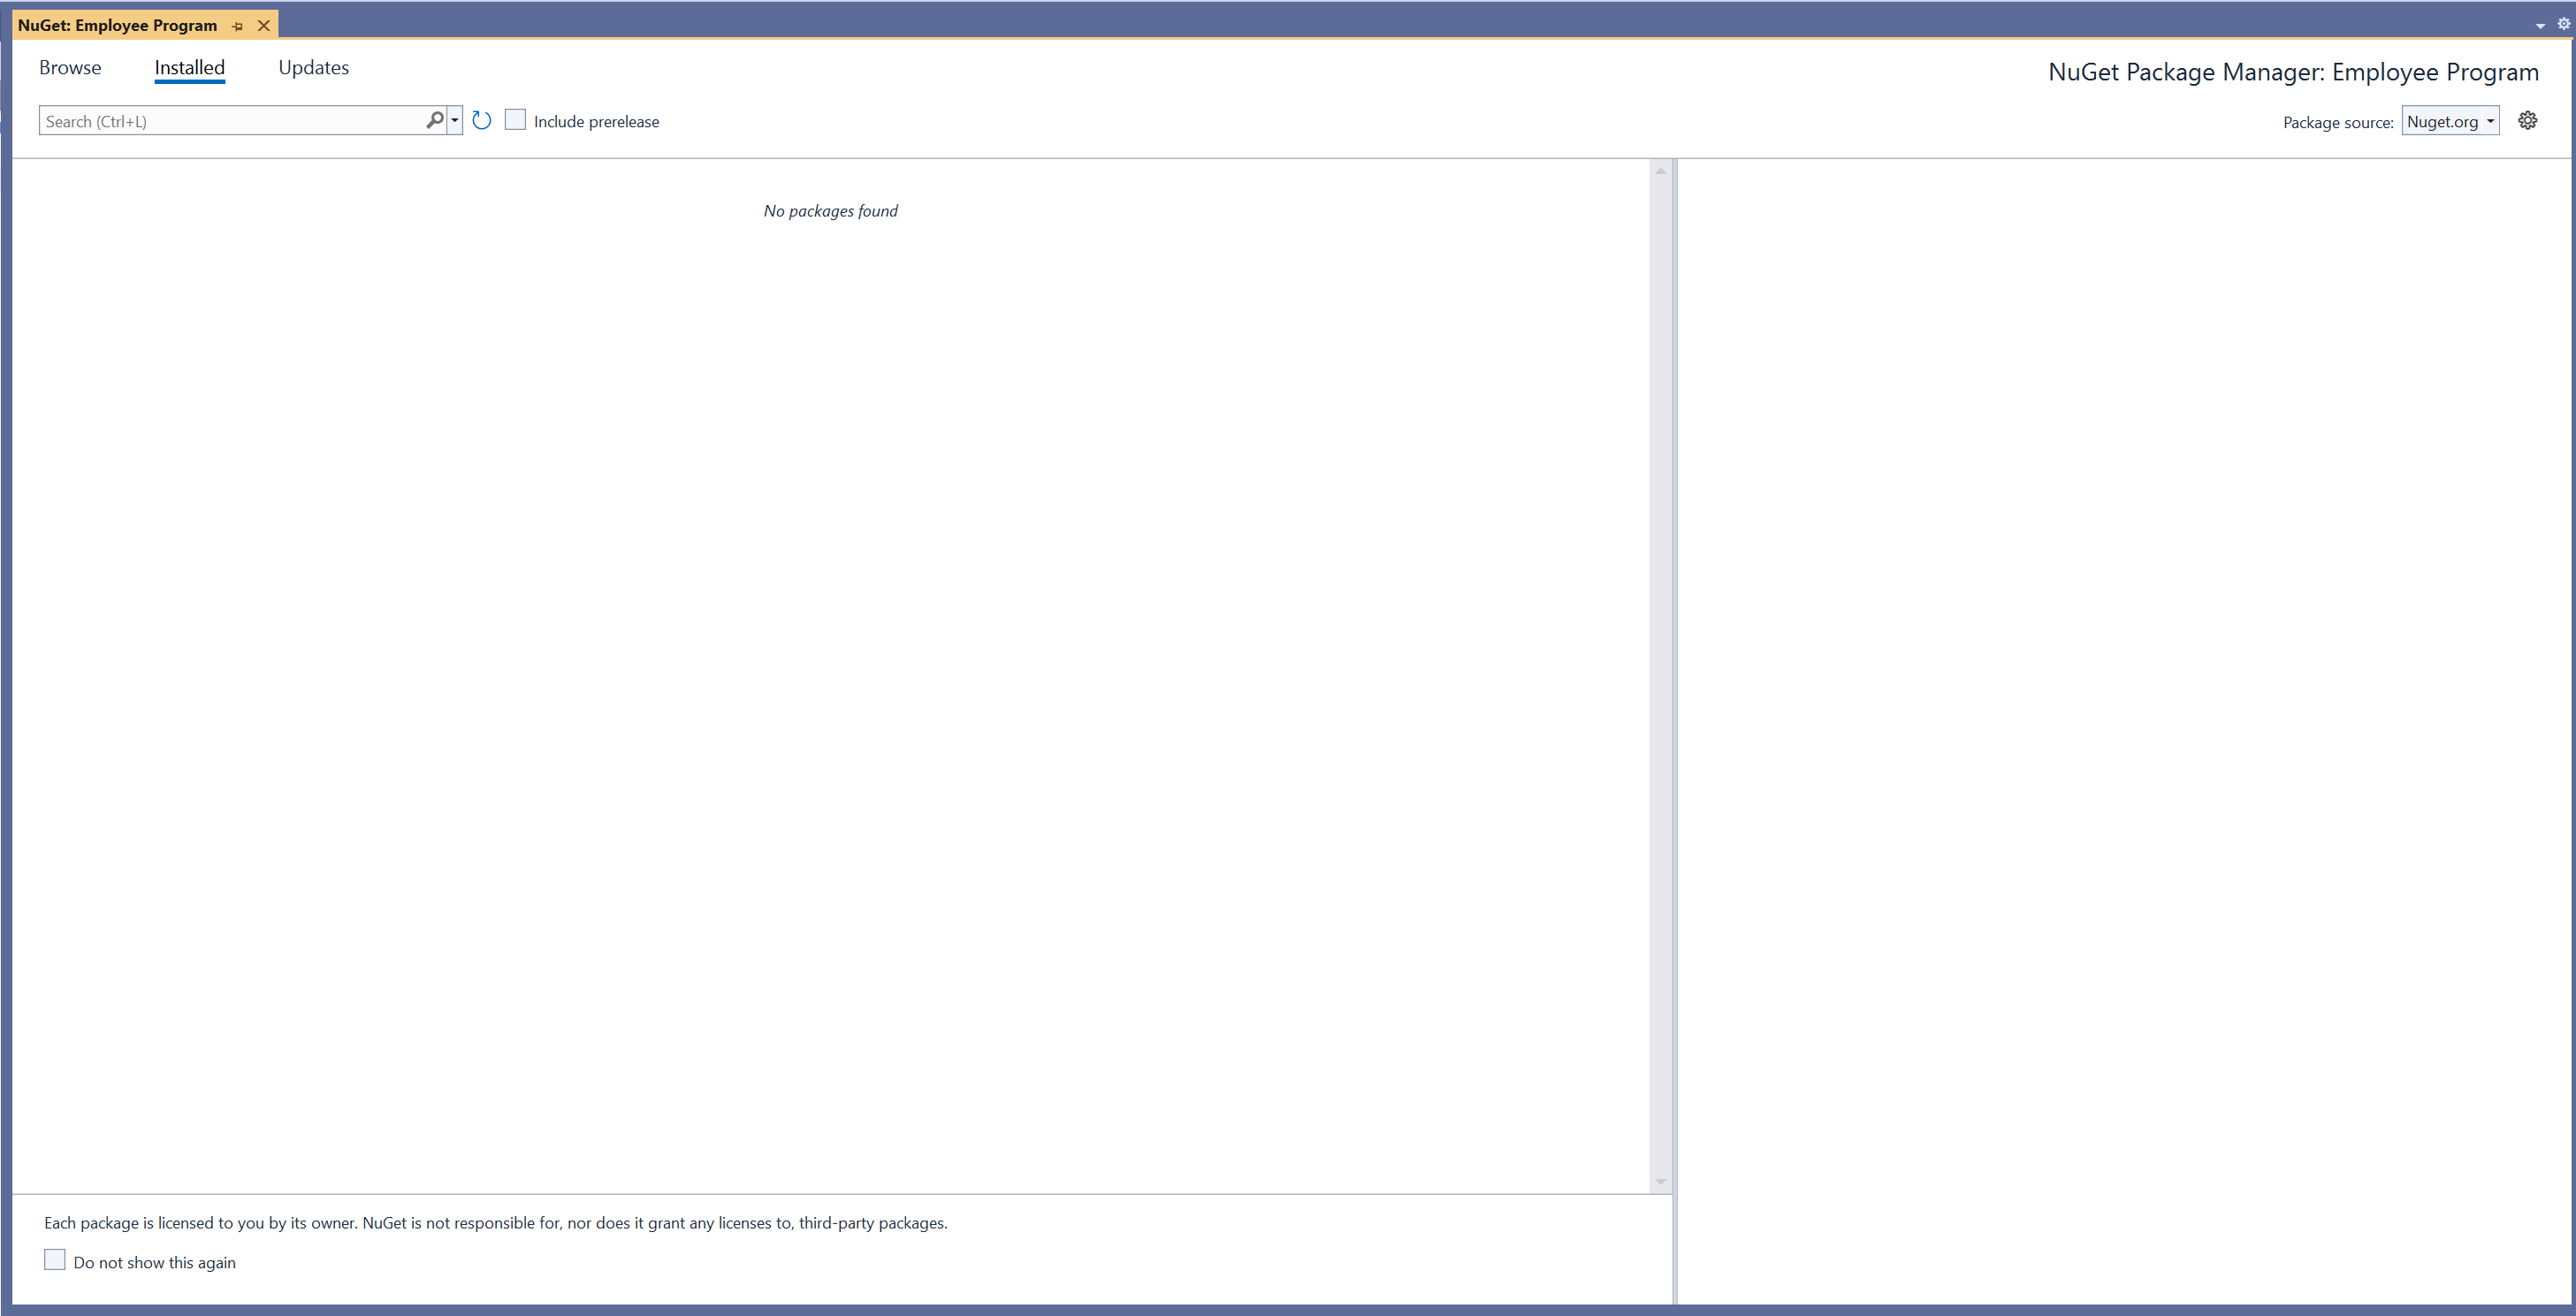
\includegraphics[scale=0.13]{nuget}
Click the "Browse" tab, and in the search box, type in "System.Data.SQLite". Look until you see this in the list:

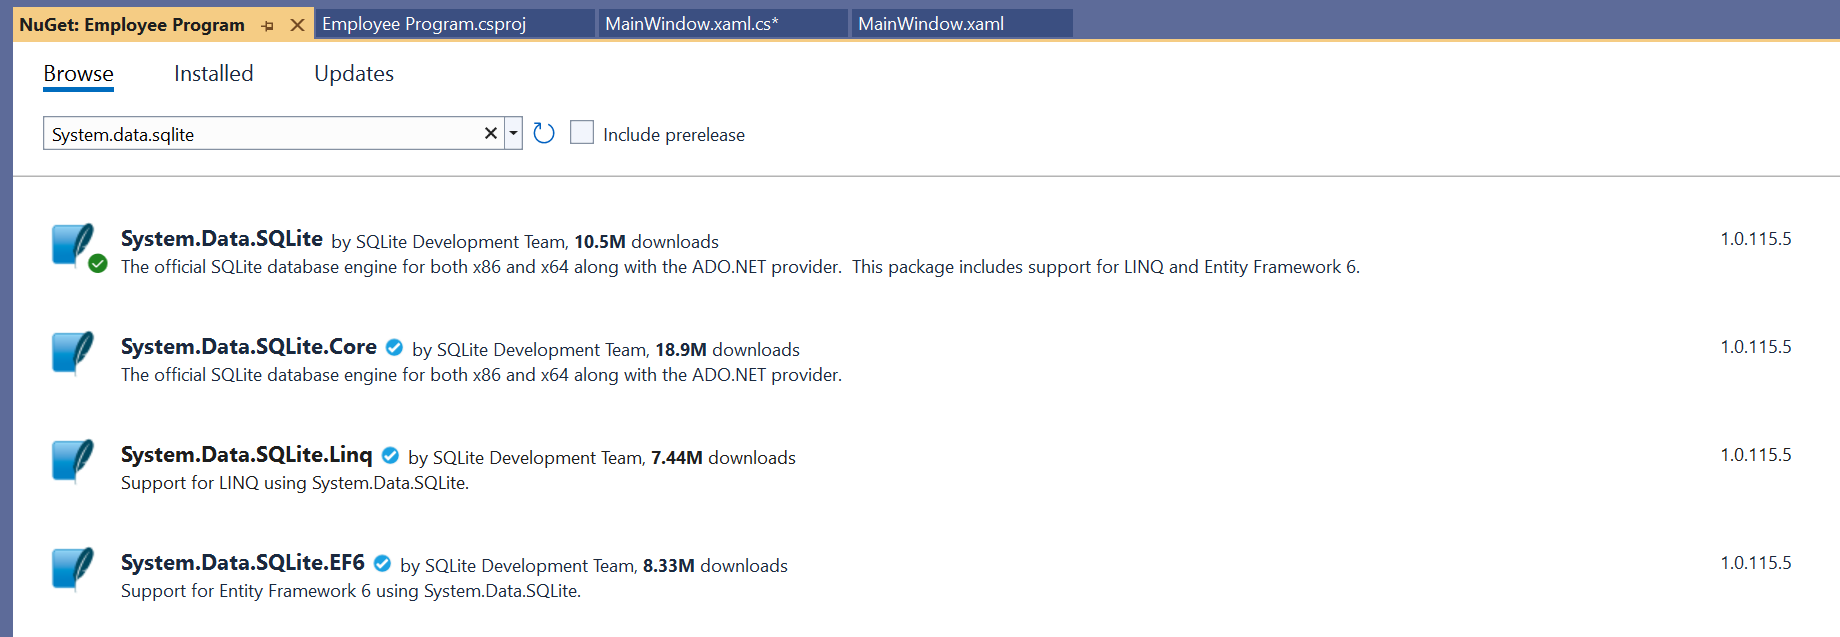
\includegraphics[scale=0.206]{sqliteinstall}

Click it, and click the "Install" button that appears on the right. Click "OK" followed by the "I Accept" buttons when they appear.

Congratulations! Now that we've installed the package, let's take a closer look at how we might want to design our database.

Relational databases are organized into \emph{tables}; each of which corresponds to a collection of related data. In our example, we might want to include a table to list our employees. Another table could list the jobs in our company. Our employee table could have information regarding the person's name and address, as well as a link to the job table that corresponds to The job table could include information about each job title, description, and pay.

When might we want to create our database? One possibility is for when our program starts. Our program can check if the database exists; if it does not, the database will be created.

If you recall from our WPF Controls chapter, WPF has events that we can set to run if a certain action occurred. We have previously considered events in the context of buttons and other controls we can add to our form, but there are actually events that can run when our form itself is loaded. One of them is the "Loaded" event, which runs if our program is started.

Let's go to our form by clicking MainWindow.xaml in the Solution Explorer. Then, click on the end of the beginning Window element, and add a Loaded attribute. I set the method name to OnProgramLoad. Then, go to the Solution Explorer and click the arrow to the left of MainWindow.xaml. Click MainWindow.xaml.cs.

We need to add a using statement to access our new SQLite features. Enter in 
\begin{CSharp}
using System.Data.SQLite;
\end{CSharp}
at the end of the list of using statements.


Add this between the brackets of our MainWindow class:
\begin{CSharp}
private void OnProgramLoad(object sender, RoutedEventArgs e)
        {

        }
\end{CSharp}
Now, let's check if our database exists. Since we're using File.Exists, let's add the requisite using statement:
\begin{CSharp}
using System.IO;
\end{CSharp}
Note that unlike with text files, our relational databases use the .sqlite extension.
\begin{CSharp}
private void OnProgramLoad(object sender, RoutedEventArgs e)
        {
            if (!File.Exists("company.sqlite"))
            {
                
            }
        }
\end{CSharp}

We want to create our database if the file does not exist. The package we installed earlier provides us with a method to create one.

\begin{CSharp}
private void OnProgramLoad(object sender, RoutedEventArgs e)
        {
            if (!File.Exists("company.sqlite"))
            {
                SQLiteConnection.CreateFile("company.sqlite");
            }
        }
\end{CSharp}
Now, we want to create the tables for our company. We need to make a connection to our database before we can work with it. The conn object needs information regarding the database name and the version number of SQLite we are using:

\begin{CSharp}
public partial class MainWindow : Window
    {
        SQLiteConnection conn = new SQLiteConnection("Data Source=company.sqlite;"
        + "Version=3");
        
        public MainWindow()
        {
            InitializeComponent();
        }

        private void OnProgramLoad(object sender, RoutedEventArgs e)
        {
            if (!File.Exists("company.sqlite"))
            {
                SQLiteConnection.CreateFile("company.sqlite");
               
                conn = new SQLiteConnection("Data Source=company.sqlite;Version=3");
            }
        }
    }
\end{CSharp}

Note that our code creates and initializes the conn variable outside of our OnProgramLoad method. That allows us to access conn inside any of our methods of our class. If the file does not exist, then conn will be empty. So, we initialize it in the method. This ensures conn always has a value when we need to use it, whether or not the database exists when we start the program.

When SQLiteConnection is first initialized, it is not actually connected to our database. We need to run our connection's Open method to do this:

\begin{CSharp}
if (!File.Exists("company.sqlite"))
            {
                SQLiteConnection.CreateFile("company.sqlite");
               
                conn = new SQLiteConnection("Data Source=company.sqlite;Version=3");

                conn.Open();
            }
\end{CSharp}
Now, we need to create tables for our database.

\begin{CSharp}
SQLiteCommand jobsTableCreate = new SQLiteCommand("CREATE TABLE jobs (title TEXT " 
+"PRIMARY KEY, description TEXT)", conn);

SQLiteCommand employeesTableCreate = new SQLiteCommand("CREATE TABLE employees" +
"(name TEXT PRIMARY KEY, address TEXT,"
                    + "title TEXT, FOREIGN KEY (title) REFERENCES jobs(title))", conn);

\end{CSharp}

(Note that the string addition is not required in your code. I used them so I could write working code that did not run off the margins of this page).

The string contents used above are SQL statements; SQL is a language we use to interact with relational databases.\footnote{This chapter will cover more basic information about SQL. For those who are interested in researching more about implementating relational databases, I suggest reading `Learning SQL, 3rd Edition', written by Alan Beaulieu and published by O'Reilly in 2020.}
Here is a basic overview on how to interpret the previous code example:

Both strings are used to create a table; we can use the CREATE TABLE feature to complete such a task. As an aside: while we capitalized those words, we could have written them in lowercase. This is equivalent:

\begin{CSharp}
SQLiteCommand jobsTableCreate = new SQLiteCommand("create table jobs (title text "+
"primary key,"description text)", conn);

SQLiteCommand employeesTableCreate = new SQLiteCommand("create table employees" + 
"(name text primary key, address text," +
"title text, foreign key (title) references " + "jobs(title))", conn);
\end{CSharp}
Using capitilized letters is the standard for SQL, so that is what we will use in this book.

Then, we use parentheses to enclose the variables we want to use in our tables. We format them as \emph{variableName variableType}. SQL does not use the term "string" to represent sequences of characters; instead, TEXT is used. PRIMARY KEY is used to set the title and name attributes as the identifiers for each row of the jobs and employees tables, respectively.

The last part of the employees string -- the part that starts with "FOREIGN KEY" -- allows us to link our two tables to each other. Specifically, we link the title property on our employees table with the corresponding property on our jobs table.

So, we've declared what our table looks like. We've also set a connection between our two tables. Before we actually add the tables to the database, we need to consider an issue with our implementation. In general, our tables would work. We could add a job in our jobs table, and add a employee in our employees table. But, what would happen if the job title would change? That would break the links between the rows in our jobs and employees table.

Our solution is to set the primary key data as an integer id, because we can expect to not modify those parts of our rows later on. So, let's revise our jobs and employees strings:
\begin{CSharp}

SQLiteCommand jobsTableCreate = new SQLiteCommand("CREATE TABLE jobs" + 
"(job_id INTEGER PRIMARY KEY " + 
"AUTOINCREMENT, title TEXT, description TEXT)", conn);

SQLiteCommand employeesTableCreate = new SQLiteCommand("CREATE TABLE employees" 
+"(employee_id INTEGER PRIMARY KEY " +
"AUTOINCREMENT, TEXT PRIMARY KEY, address TEXT, "
+ "title TEXT, FOREIGN KEY (title) REFERENCES jobs(title))", conn);
\end{CSharp}

The AUTO INCREMENT property prevents us from needing to worry about setting an id when we add data to our tables. What it does is set the id to be the id of the previous element, plus one.

Now, let's add these tables to our database:
\begin{CSharp}
jobsTableCreate.ExecuteNonQuery();
employeesTableCreate.ExecuteNonQuery();
\end{CSharp}
Whenever we are done using a database in a method, we use the close method of our connection object to close the connection.

\begin{CSharp}
conn.Close();
\end{CSharp}
\section{Inserting data}
\index{INSERT INTO}
SQL has the \emph{INSERT INTO} keyword that allows us to insert in data into our database tables.

For example:
\begin{CSharp}

string jobName = "Frontend Web Developer"
string jobDescription = "This job concerns"+
"developing the client-side part of our website using HTML, CSS, and JavaScript."
    
SQLiteCommand insertJob = new SQLiteCommand("INSERT INTO JOBS "+ "(title, description) "
+"VALUES (?,?)", conn);

insertJob.Parameters.Add(jobName);
insertJob.Parameters.Add(jobDescription);

insertJob.ExecuteNonQuery();
\end{CSharp}
In the above code, the question marks correspond to the different parameters in our query. We set our variables that the query is using with the Parameters.Add method. So, our query effectively becomes this:

\begin{verbatim}
    INSERT INTO JOBS (title, description)
VALUES (Frontend Web Developer, This job concerns developing the client-side
part of our website using HTML, CSS, and JavaScript.
\end{verbatim}

Note: If you get an exception and have to fix a typo when writing this code, be sure to delete the company.sqlite file before you try running the program again. Recall that this table creation code only runs if the database file doesn't exist.


Inserting data into the Employee table is more difficult as we need to obtain an id of the job that a person is a part of. We will consider this soon.
\exercise
Create a Console program that creates a database with a table that contains an id and a text field  named "word". Allow the user to insert in words. After the user types in a word and presses enter, insert the word into our database. Continue until the user enters in a blank line. When that happens, close the connection.

When you're done testing your program, go back to our WPF program.
\section{Retrieving Data}
\index{SELECT}
\index{FROM}
Suppose we wanted to obtain all of the job titles from our jobs table. We could use the SQLiteDataReader class to get this:

\begin{CSharp}

//First, create our query
SQLiteCommand getJobs = new SQLiteCommand("SELECT title FROM jobs");

//Then, use the SQLiteDataReader class to obtain the results.
//This functions similarly to using a StreamReader.

using (SQLiteDataReader reader = getJobs.ExecuteReader();
{
  while (reader.Read())
  {
   
  }
}
\end{CSharp}
Our `reader' variable is an array that represents the returned values from ExecuteReader. Each time Read() is called in the while loop, the array is initialized to the next row of our table. We can use ToString() to get the string representation of a value at a particular index.

\exercise
Use a SQLiteDataReader to output the data from the previous exercise.
\par\noindent\rule{\textwidth}{0.4pt}
\index{ORDER BY}
SELECT can actually be used pretty similarly to LINQ. For example, if we wanted to order our results by length:

\begin{CSharp}
SQLiteCommand getJobsOrdered = new SQLiteCommand("SELECT title FROM jobs "
+ "ORDER BY length(title)");
\end{CSharp}
\exercise
In our WPF program, create two textboxes for a name and address, as well as a button. When the user presses the button, obtain the contents of the two boxes and insert the values into the database, assuming the person being added is a "Frontend Web Developer". Hint: You need to determine the id of a web developer before you can add a user.
\chapter{Introduction to Git and GitHub}
\minitoc
In the development process, it is useful to be able to make backups of your program and allow other developers to easily access it so they can make their own changes. This final chapter concerns two technologies that facilitate this: Git and GitHub.

\section{Why use Git and GitHub?}
I mentioned two primary reasons to use Git earlier:
\subsection{Backups}
When we make programs, we are liable to make mistakes. Sometimes, we don't notice these errors only until after we've saved our program, exited our development environment, and forgotten what specific code edits we made. What could we do to go back to our previous code?
\index{Git}
Without a \emph{version control system} such as Git, there isn't much recourse. Perhaps you made a copy of your program folders so you could access that earlier version: before you made a mistake. But even then, this is a risky proposition. You have to specifically recall to make copies of your program. You have to find a place to store it on your computer, and try to label them so you know which folder corresponds to which version of your program. Even in the best case scenario -- where you diligently create backups every time you make a change -- you have the risk of running out of storage from all your backups.
\subsection{Collaboration}
With version control software such as Git, businesses can store their programs on an external server that other users can get data from for their computer and send data to. Git makes it easy to manage and sync each individual's work on a program.

\noindent\rule{12.5cm}{0.4pt}
Git is a program that is used to make and manage \emph{git repositories}. Git repositories consist of a user-made program, as well as special folders created by the Git program to manage program versions.

Git makes the process of managing program versions much easier. Instead of trying to create copies of folders, git allows us to manage program versions from Windows's command line. Furthermore, all of your versions are kept in a single folder structure, and Git only creates new versions of files when those particular files have been changed.
\section{Installing and Initializing Git}
Git can be downloaded from the \href{https://git-scm.com/}{Git website.} Follow the installation instructions for your particular operating system.

Now that you've gotten Git installed, let's explore using it with a small program. Create a console program called "Hello World", and note where the project is saved to. 
Write a program that outputs, "Hello, Git!" to the screen.

\begin{CSharp}
Console.WriteLine("Hello, Git!");
\end{CSharp}
Now, we need to open our folder in our command line. If you're using Windows:
Press the Windows key, type in "Command Prompt", and press enter.

The command prompt has text describing what folder it is currently in (you can think of this like the File Explorer, except we're navigating through and opening folders through a Console interface -- not a graphical user interface). For example, for me, it is:
\begin{verbatim}
C:\Users\alex
\end{verbatim}
\index{cd command}
We need to change to the folder where our program is located. We can use the \emph{cd} command to do this. Type in "cd" into the command prompt, press space, and write the name of the folder, enclosed in quotes.\footnote{Note that we do not have to use quotes if the path to the folder does not have spaces.}For example, I would type in:
\begin{verbatim}
cd "C:\Users\alex\source\repos\Hello World"
\end{verbatim}
Now we can set up our git repository.
First, type in:
\begin{verbatim}
    git init
\end{verbatim}
There we go; we've initialized git for our project. Let's edit our program.

\exercise
Change the text in our program to a new string.
\par\noindent\rule{\textwidth}{0.4pt}
Now, we need to let git know which of our files we want to save.
\index{git!add}
In our command line, type in
\begin{verbatim}
    git add .
\end{verbatim}
then press ENTER.
To actually save, or \emph{commit} these files, type,
\index{git!commit}
\begin{verbatim}
    git commit -m "First commit"
\end{verbatim}
We didn't have to specifically write "First commit" there. Use anything that you think will describe the update you made. Press ENTER after you're done.
\index{git log}
How can we revert back to a previous version? There is a command to do this, but we need to get an identifier for the commit that we want to revert to. First, exit Visual Studio. Type in 
\begin{verbatim}
    git log
\end{verbatim}

You'll see all of the various versions you've set up. Find the one that corresponds to the version you want, then type
\index{git checkout}
\begin{verbatim}
    git checkout (version number)
\end{verbatim}
The version number to use is displayed right after the word "commit" in the listing in the git log. If you open Visual Studio, you'll see the previous version of your file.

Suppose you were collaborating with other people, and you need to obtain a copy of the folder structure of the current version they are working on. There are two git commands that are useful in this situation; pull and push. \emph{pull} is used to obtain the latest version of a project, while \emph{push} is used to put your version onto a server.

We will talk about this more in the context of GitHub.

\section{Setting up GitHub}
\index{GitHub}
GitHub is a website that is used to store git repositories. Since repositories are stored online, it is easy to collaborate with others who are not in the same area. GitHub isn't a bare-bones website for downloading git repositories; users can file bug reports, contribute to discussions, and easily browse the website to look for programs they find interesting or useful. This makes the website especially a boon for open-source software development, where individuals or other groups can contribute to the writing of a program.
\exercise
Go to \href{https://github.com/}{https://github.com/} and make a GitHub account.

\noindent\rule{12.5cm}{0.4pt}
Now, let's save our project to GitHub. To do this, we need to create a repository on the website, and \emph{push} our project to it.

Go to github.com and click "New" at the left:

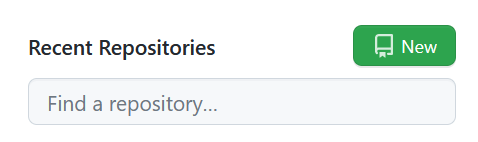
\includegraphics[scale=0.206]{githubnewrepo}

Then, on the next screen, type in your repository name. Click "Private" if you don't want others to view your repository. Then, click "Create Repository".

Follow the instructions listed on the page to push to your git repository.
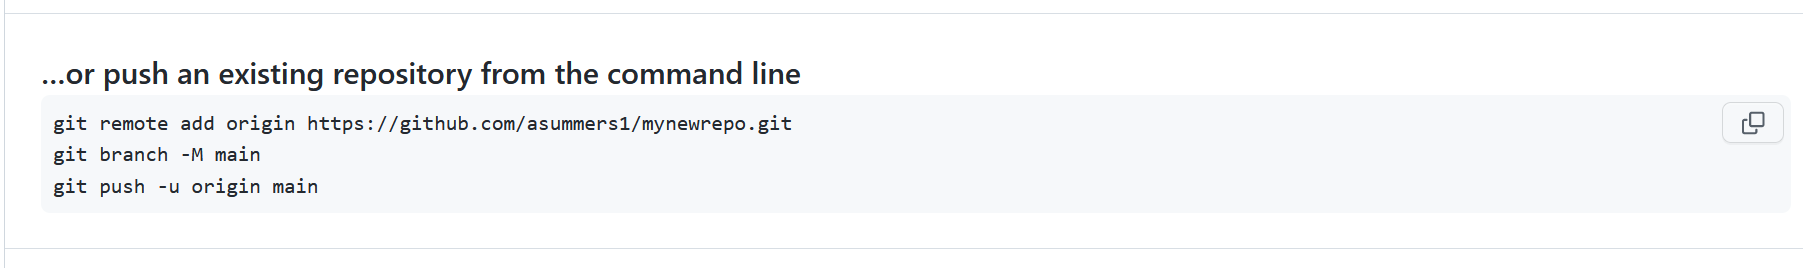
\includegraphics[scale=0.2]{GitHubInstructions}
\exercise

The "pull" command takes a url (ending in .git) to pull changes from GitHub. Make a change to your program, push it to GitHub, and pull it.
\exercise
Try exploring some of the publicly-available repositories on GitHub. If you see a C\# console program or a WPF program, try pulling it and making your own changes.
\section{Where to Go From Here}
Congratulations! You're at the end of the book. Where should you go from here? It depends on what you want to work with!

\subsection{Desktop Programming}
Try making projects with WPF. I recommend thinking of a topic that would interest and challenge you, so you can increase your understanding of the technology while being driven to succeed. Perhaps you could think of a situation where you're missing a program that would make your life easier. If you get stuck, or otherwise want to learn more, be sure to read through Microsoft's WPF documentation.
\subsection{Web Design}
\index{ASP.NET}
Web programming using C\# predominantly uses ASP.NET. \href{https://docs.microsoft.com/en-us/aspnet/core/?view=aspnetcore-6.0}{Microsoft has a lot of documentation} on how to use the technology. If you prefer a book \emph{ASP.NET Core in Action, Second Edition} is highly-rated.
\subsection{Game Development}
\index{Unity}
The Unity framework is very popular for making 2D and 3D video games. Unity (the company that makes Unity) has a \href{https://docs.unity.com/}{great amount of documentation on their website}. If you want a textbook, I've read a few chapters of "Unity in Action, Third Edition" and liked it.
\backmatter
\printindex
\end{document}